\documentclass[a4paper, 12pt]{article}

\usepackage{custom}

%--------------------VARIABILI--------------------
\def\lastversion{v1.0}
\def\title{Norme di progetto}
\def\date{17 Marzo 2025}
%------------------------------------------------

\begin{document}

\primapagina

\begin{registromodifiche}
    \lastversion & 17 Marzo 2025 &  & Enrico Bianchi & Release\\
    \hline
        v0.15 & 16 Marzo 2025 & Enrico Bianchi & Francesco Savio & Verifica generale e correzioni\\
    \hline
        v0.14 & 27 Febbraio 2025 & Marko Peric & Francesco Savio & Scrittura sezioni: \hyperref[par:staruml]{StarUML}, \hyperref[par:requisiti_software]{Requisiti Software}\\
    \hline
        v0.13 & 9 Gennaio 2025 & Enrico Bianchi, Matteo Eghosa & Marko Peric & Scrittura sezione: \hyperref[subsec:accertamento_qualità]{Processo di accertamento qualità}\\
    \hline
        v0.12 & 8 Gennaio 2025 & Pedro Leoni & Marko Peric & Modifica sezione: \hyperref[par:casi_uso]{Casi d'uso}, \hyperref[subpar:comandi_personalizzati]{Comandi personalizzati}, \hyperref[subpar:ambienti_personalizzati]{Ambienti personalizzati}\\
    \hline    
        v0.11 & 7 Gennaio 2025 & Marko Peric & Enrico Bianchi & Modifica sezione: \hyperref[subpar:tabelle]{Creazione delle tabelle}, Aggiunta sezione: \hyperref[subpar:grafici]{Creazione dei grafici}\\
    \hline
        v0.10 & 31 Dicembre 2024 & Marko Peric & Francesco Savio & Modifica sezioni: \hyperref[par:calcolo_ore_lavoro]{Github action controllo delle ore di lavoro}, \hyperref[par:correzione_grammaticale]{Github action del controllo ortografico dei documenti LaTeX}\\
    \hline
        v0.9 & 26 Dicembre 2024 & Marko Peric & Enrico Bianchi & Modifica sezione: \hyperref[subsec:documentazione]{Documentazione}, introdotta descrizione \hyperref[subsec:struttura_piano]{struttura documento Piano di Progetto}\\
    \hline
        v0.8 & 23 dicembre 2024 & Francesco Savio & Marko Peric & Modifica sezione: \hyperref[sec:Processi_di_supporto]{Processi di supporto}, \hyperref[subsec:proc_infrastruttura]{Processo di infrastruttura}\\ 
    \hline
        v0.7 & 22 dicembre 2024 & Enrico Bianchi, Guirong Lan & Marko Peric & Scrittura sezione: \hyperref[subsec:proc_verifica]{Processo di Verifica}\\
    \hline
        v0.6 & 21 dicembre 2024 & Guirong Lan & Marko Peric & Scrittura sezione: \hyperref[sec:Processi_Primari]{Descrizione Processi Primari}, \hyperref[subsection:Processo_acquisizione]{Processo di acquisizione}, \hyperref[subsection:processo_fornitura]{Processo di fornitura}\\ 
    \hline
        v0.5 & 11 dicembre 2024 & Pedro Leoni & Francesco Savio, Enrico Bianchi & Scrittura sezione: \hyperref[subsec:documentazione]{Documentazione}\\  
    \hline
        v0.4 & 11 dicembre 2024 & Pedro Leoni & Francesco Savio, Enrico Bianchi & Scrittura sezione: \hyperref[subsec:gestione_della_configurazione]{Gestione della configurazione}\\  
    \hline
        v0.3  & 11 dicembre 2024 & Pedro Leoni, Francesco Savio & Francesco Savio, Enrico Bianchi & Scrittura sezione: \hyperref[subsec:proc_infrastruttura]{Processo di infrastruttura}\\  
    \hline
        v0.2 & 11 dicembre 2024 & Pedro Leoni, Enrico Bianchi & Francesco Savio, Enrico Bianchi & Scrittura sezione: \hyperref[subsec:gestione_progetto]{Gestione di progetto}\\  
    \hline
        v0.1 & 11 dicembre 2024 & Pedro Leoni, Francesco Savio, Matteo Eghosa & Francesco Savio, Enrico Bianchi & Scrittura sezione: \hyperref[subsection:processo_sviluppo]{Processo di sviluppo}\\  
    \hline
\end{registromodifiche}

\tableofcontents

\newpage

\section{Processi primari}
\label{sec:Processi_Primari}
I processi primari definiti dalla norma \glossario{ISO/IEC 12207} sono essenziali per la realizzazione di un progetto e sono strettamente legati all'acquisizione, alla realizzazione, alla gestione, all'operazione e al ritiro del software durante l'intero \glossario{ciclo di vita}. 
Un processo primario consiste in un insieme di attività fondamentali e interconnesse, e variano a seconda della tipologia di processo.
Questi processi sono cruciali nelle fasi operative del \glossario{ciclo di vita} del software e sono determinanti per garantire una produzione, manutenzione e dismissione in modo efficace. La norma distingue cinque principali processi primari, ognuno dei quali comprende attività chiave per lo sviluppo e la gestione del software, dalla sua concezione fino al suo ritiro.
I cinque processi sono:
\begin{enumerate}
    \item \textbf{Processo di acquisizione}; 
    \item \textbf{Processo di fornitura}; 
    \item \textbf{Processo di sviluppo};
    \item \textbf{Processo di operazione}; 
    \item \textbf{Processo di manutenzione};
\end{enumerate}
\textbf{Nota bene}: Per la questione didattica il processo di manutenzione non verrà implementato.

\subsection{Processo di acquisizione}
\label{subsection:Processo_acquisizione}
Il processo di acquisizione, secondo la norma ISO/IEC 12207, comprende l'insieme delle attività che un'organizzazione, cioè il \glossario{Fornitore}, deve svolgere per ottenere un sistema, un prodotto software o un servizio software. Esso prevede l'identificazione dei requisiti, la selezione di un Fornitore e un \glossario{Proponente}, la stipula di un contratto, la supervisione della fornitura e, infine, l'accettazione e il completamento del prodotto o servizio acquisito.
Dunque, per il nostro gruppo, il processo di acquisizione consiste nelle seguenti attività principali:

\begin{itemize}
    \item \textbf{Iniziazione}; 
    \item \textbf{Studio di fattibilità}; 
    \item \textbf{Selezione del capitolato}; 
    \item \textbf{Preparazione della candidatura}; 
    \item \textbf{Accettazione della candidatura}; 
\end{itemize}

\subsubsection{Iniziazione}
Il Fornitore effettua un'analisi preliminare dei capitolati d’appalto, la comprensione degli obiettivi e dei requisiti iniziali per lo sviluppo, includendo il confronto e la discussione con i proponenti.

\subsubsection{Studio di fattibilità}
Il Fornitore analizza i capitolati per identificare eventuali punti critici e valuta le idee ricevute dai proponenti.

\subsubsection{Selezione del capitolato}
Il Fornitore sceglie e prepara il capitolato d'appalto che meglio soddisfa le sue aspettative.

\subsubsection{Preparazione della candidatura}
Il Fornitore prepara e definisce la redazione dei documenti necessari:
\begin{itemize}
    \item \textbf{Lettera di candidatura};
    \item \textbf{Stima dei costi};
    \item \textbf{Assunzione d’impegni};
    \item \textbf{Valutazione dei capitolati}.
\end{itemize}
Revisionando il contenuto per correggere eventuali errori e, se necessario, aggiorna il documento prima della presentazione ai \glossario{Committenti}.

\subsubsection{Accettazione della candidatura}
L'approvazione della soluzione selezionata e la conseguente formalizzazione del contratto spettano ai committenti, i quali, con la loro approvazione, rendono ufficiale il contratto.

\subsection{Processo di fornitura}
\label{subsection:processo_fornitura}
Il processo di fornitura, definito dalla norma ISO/IEC 12207, comprende le attività svolte dal Fornitore e inizia con la presentazione di una proposta al Proponente o la stipula di un contratto. Nel nostro caso, il processo riguarda la Proponente Zucchetti S.p.A. e si avvia al termine del processo di acquisizione, ossia al completamento della fase di accettazione della candidatura.
Il processo prevede la pianificazione e l’organizzazione delle risorse, delle procedure e dei piani necessari per la gestione del progetto, fino alla consegna del sistema, prodotto o servizio software. Questo processo è fondamentale per garantire che il software soddisfi i requisiti del cliente, sia di alta qualità e venga realizzato rispettando tempi e costi concordati. L’obiettivo principale è allineare costantemente le aspettative dell’acquirente con i risultati ottenuti durante l’esecuzione del progetto.
Dunque, per il nostro gruppo, il processo si articola nelle seguenti attività principali:
\begin{itemize}
    \item \textbf{Pianificazione};
    \item \textbf{Esecuzione e controllo};
    \item \textbf{Revisione e valutazione};
    \item \textbf{Consegna e completamento};
\end{itemize}

\subsubsection{Pianificazione}
Il Fornitore definisce obiettivi, risorse e procedure necessari per l’esecuzione del progetto, identificando i requisiti per la gestione, la misurazione della qualità e lo svolgimento delle attività. Questa fase sta principalmente nella redazione del Piano di Progetto, che pianifica l’utilizzo delle risorse e documenta i risultati attesi.

\subsubsection{Esecuzione e controllo}
Il Fornitore attua le attività pianificate nel Piano di Progetto, rispettando le norme stabilite. Inoltre, viene effettuato un controllo continuo sullo stato di avanzamento e sulla gestione delle risorse, garantendo la rendicontazione rispetto agli obiettivi prefissati. 

\subsubsection{Revisione e valutazione}
Il Fornitore definisce criteri e procedure per la revisione ed esegue le operazioni in conformità a tali criteri. L'obiettivo è verificare che il progetto soddisfi i requisiti e rispetti gli standard stabiliti.

\subsubsection{Consegna e completamento}
Consegna del progetto, verifica finale e accettazione da parte dell’acquirente.

\subsubsection{Contatti con la Proponente dell’azienda}
La Proponente, Zucchetti S.p.A., fornisce l'indirizzo email del proprio rappresentante per la comunicazione asincrona e per la pianificazione di videochiamate su Google Meet con il Fornitore. Le comunicazioni tra Proponente e Fornitore riguardano vari aspetti del progetto, tra cui la raccolta dei requisiti, la raccolta di feedback sui risultati ottenuti e le indicazioni sull'avanzamento del progetto. Durante il corso del progetto, che ha carattere didattico, la Proponente assume il ruolo di cliente, mantenendo un ampio grado di libertà per il Fornitore, il quale è responsabile della realizzazione del prodotto. Per ogni colloquio con l'azienda Proponente, ovvero per ogni videochiamata tramite Google Meet, sarà redatto un Verbale Esterno che riassume i punti chiave discussi durante l'incontro.

\subsubsection{Documentazione fornita}
Di seguito viene descritta la documentazione che il gruppo rende disponibile alla Proponente Zucchetti S.p.A. e ai committenti, Prof. Tullio Vardanega e Prof. Riccardo Cardin.

\paragraph{Piano di progetto}
Il Piano di Progetto è un documento redatto dal responsabile del progetto, che fornisce una visione dettagliata della gestione e dell’organizzazione del gruppo di lavoro. La sua funzione principale è quella di pianificazione, monitoraggio e controllo delle attività, al fine di garantire il raggiungimento degli obiettivi nei tempi e nei costi stabiliti. Inoltre, il piano include l'analisi e la gestione dei rischi, nonché la pianificazione, il preventivo e il consuntivo di ciascun sprint, monitorando costantemente l'avanzamento del progetto e le risorse utilizzate.
Il documento è suddiviso nelle seguenti sezioni:
\begin{itemize}
    \item \textbf{Introduzione}: Una breve descrizione dello scopo del documento e delle varie sezioni che lo compongono.
    \item \textbf{Analisi dei rischi}: Riguarda l'identificazione dei potenziali rischi che potrebbero sorgere durante il corso del progetto, i quali potrebbero causare ritardi o ostacoli nella sua progressione. Vengono inoltre sviluppate strategie di prevenzione per evitare che tali rischi si manifestino, nonché strategie di mitigazione per ridurne l'impatto nel caso in cui si verificassero, al fine di garantire la continuità del progetto.
    \item \textbf{Stima dei costi}: Calcolo delle risorse necessarie per il completamento del progetto, che viene aggiornato ad ogni sprint.
    \item \textbf{\glossario{Milestone} principali}: Sezione dedicata all'indicazione delle milestone fondamentali e delle baseline di riferimento del progetto.
    \item \textbf{Primo periodo}: Rappresenta la fase iniziale del gruppo.
    \item \textbf{\glossario{Sprint}}: Gli sprint rappresentano fasi del progetto in cui vengono definiti obiettivi specifici e attività da completare. Durante ogni sprint, il gruppo si impegna a raggiungere tali obiettivi. Inoltre, si stabiliscono una revisione retrospettiva e la data per lo sprint successivo.
    La sottosezione si articola nelle seguenti parti:
    \begin{enumerate}
        \item \textbf{Obiettivi}: Definisce gli obiettivi specifici dello sprint.
        \item \textbf{Pianificazione}: Presenta il preventivo dei costi e delle risorse previste per lo sprint.
        \item \textbf{Consuntivo}: Riporta il resoconto dei costi e delle risorse effettivamente utilizzati.
        \item \textbf{Retrospettiva}: Riporta la conclusione dello sprint e propone miglioramenti sui punti deboli emersi.
        \item \textbf{Aggiornamento risorse rimaste}: Aggiorna la situazione delle risorse disponibili per il progetto.
    \end{enumerate}
\end{itemize}

\paragraph{Analisi dei requisiti}
L’analisi dei requisiti è un documento redatto dall’analista che fornisce una visione chiara delle richieste e delle aspettative dell’azienda Proponente. Va ad includere un elenco dettagliato delle funzionalità da sviluppare e implementare, nonché i casi d’uso che definiscono le interazioni tra il sistema e l’utente.
Il documento è suddiviso nelle seguenti sezioni:
\begin{enumerate}
    \item \textbf{Introduzione}: Una breve descrizione dello scopo del documento e delle varie sezioni che lo compongono.
    \item \textbf{Descrizione del prodotto}: Descrive gli obiettivi del prodotto, le sue funzioni principali e le caratteristiche.
    \item \textbf{Casi d’uso}: Indica tutti i casi d’uso individuati dal gruppo durante analisi.
    \item \textbf{Requisiti}: Elenco completo dei requisiti del prodotto, organizzato per categorie e con riferimento alle fonti da cui proviene il tracciamento.
\end{enumerate}

\paragraph{Piano di Qualifica}
Il Piano di Qualifica è un documento che definisce le attività del verificatore nel progetto, stabilendo le strategie e gli approcci per garantire la qualità del prodotto software in fase di sviluppo. Redatto dal verificatore, questo documento descrive le modalità di verifica e validazione. Tutti i membri del team si baseranno su questo documento per garantire il raggiungimento della qualità desiderata.
Il documento è suddiviso nelle seguenti sezioni: 
\begin{enumerate}
    \item \textbf{Introduzione}: Una breve descrizione dello scopo del documento e delle varie sezioni che lo compongono.
    %\item \textbf{Obiettivi di qualità}: Questa sezione presenta i valori accettabili e gli ambiti per le metriche definite dal team, le metriche sono divise:Qualità di processo,Qualità di prodotto,Qualità per obiettivo.
    %\item \textbf{Metodologie di testing}: Include tutti i test necessari per verificare che il prodotto rispetti i requisiti specificati.
    %\item \textbf{Cruscotto di valutazione della qualità}: Vengono scritte tutte le attività di verifica effettuate e le problematiche emerse durante lo sviluppo del software.
\end{enumerate}

\paragraph{Glossario}
Il Glossario è un elenco dettagliato e organizzato di tutti termini, acronimi e definizioni utilizzati nella documentazione. L’obiettivo principale di questo documento è fornire una comprensione chiara dei concetti e dei termini specifici impiegati nel progetto, garantendo una comunicazione coerente e precisa tra tutti i membri del gruppo e con gli \glossario{Stakeholder}. In questo modo, si facilita il lavoro collaborativo e si assicura un allineamento efficace su linguaggio e significati durante l'intero ciclo di vita del progetto.

\paragraph{Lettera di presentazione}
La Lettera di Presentazione è il documento con cui il gruppo comunica la propria candidatura alle revisioni di avanzamento \glossario{Requirements and Technology Baseline} e \glossario{Product Baseline}. Nel primo caso essa include informazioni sui repository di documentazione e codice sorgente, il riferimento al \glossario{Proof of Concept} e un aggiornamento sugli impegni con la stima del preventivo "a finire". 

\subsection{Processo di sviluppo}
\label{subsection:processo_sviluppo}
ll processo di sviluppo riguarda l'insieme di attività necessarie per produrre e implementare il software, assicurandosi che risponda ai requisiti definiti e sia di qualità adeguata.

\subsubsection{Analisi dei requisiti}
L'analisi dei requisiti è una attività cruciale nel ciclo di vita del software, in cui vengono raccolte, analizzate e documentate le esigenze degli stakeholder per definire chiaramente cosa il sistema dovrà fare. 
Questa attività produce il documento di analisi dei requisiti descritto nella sezione \hyperref[subsec:documentazione]{Documentazione}.

\paragraph{Requisiti}
I requisiti vengono categorizzati in:
\begin{enumerate}
    \item \textbf{Requisiti funzionali}.
    
    Rappresentano ciò che un sistema deve fare per soddisfare le esigenze degli utenti o degli stakeholders.

    \item \textbf{Requisiti qualitativi}.
    
    I requisiti di qualità (requisiti non funzionali) descrivono caratteristiche qualitative del sistema, come prestazioni, sicurezza, usabilità e manutenibilità.

    \item \textbf{Di vincolo}.
    
    I requisiti di vincolo rappresentano limitazioni o condizioni obbligatorie che influenzano lo sviluppo, l'implementazione o l'operatività del sistema. 
    A differenza dei requisiti funzionali o di qualità, non descrivono cosa deve fare il sistema, ma come deve essere realizzato rispettando regole o restrizioni specifiche. 

    \item \textbf{Prestazionali}.
    
    I requisiti prestazionali sono un tipo specifico di requisiti non funzionali che definiscono le aspettative relative alle prestazioni del sistema.
    Alcuni esempi sono: la velocità, il tempo di risposta, la capacità di carico, e altre caratteristiche misurabili legate all'efficienza.
\end{enumerate}


\paragraph{Casi d'uso}
I casi d'uso forniscono una descrizione dettagliata delle funzionalità del sistema dal punto di vista degli utenti, delineando come il sistema risponda a specifiche azioni o scenari. 
In particolare un caso d'uso rappresenta un uso completo del sistema dalla prospettiva dell'utente.
I casi d'uso vengono rappresentati tramite una combinazione di descrizione e diagramma UML.
Durante la definizione di un caso d'uso possono emergere nuove informazioni che richiedono una modifica dei casi d'uso definiti in precedenza.
La definizione dei casi d'uso non è quindi lineare.

\subparagraph{Descrizione}
Nella \hyperref[tab:template_casi_uso]{Tabella \ref{tab:template_casi_uso}} viene mostrato il template per la descrizione dei casi d'uso.
Ogni descrizione di caso d'uso deve includere:
\begin{enumerate}
    \item \textbf{Identificativo}.
    
    \texttt{UC-<ID caso principale>.<ID sotto caso>}. 
    
    Dove:
    \begin{enumerate}
        \item \texttt{<ID caso principale>}: identificativo numerico del caso d'uso principale (numero crescente).

        \item \texttt{<ID sotto caso>}: identificativo numerico del sotto caso d'uso (presente solo se si tratta di un sotto caso d'uso).
    \end{enumerate}

    \item \textbf{Pre-condizioni}.
    
    Stato iniziale del sistema o vincoli necessari per l'attivazione del caso d'uso.

    \item \textbf{Post-condizioni}.
    
    Stato finale del sistema dopo un esecuzione normale(priva di errori) del caso d'uso.

    \item \textbf{Post-condizioni errore}.
    
    Stato finale del sistema dopo un esecuzione fallita del caso d'uso.

    \item \textbf{Attori}.
    Un attore è un entità esterna(\underline{umana o meno}) al sistema che interagisce con il sistema per iniziare o per contribuire al compimento l'esecuzione di un caso d'uso.  
    Gli attori si dividono in:
    \begin{enumerate}
        \item  \textbf{Attori primari}: attori principali che partecipano al caso d'uso, solitamente contengono gli attori che iniziano l'interazione e/o sono i destinatari delle informazioni in output del caso d'uso.
        \item \textbf{Attore secondario}: altri attori coinvolti che non sono protagonisti nell'esecuzione del caso d'uso(es. Sistemi esterni).
    \end{enumerate}

    \item \textbf{Trigger}.
    
    Evento eseguito da un attore che attiva il caso d'uso.
    
    \item \textbf{User story}.
    
    Una breve descrizione di una funzionalità del software, scritta dal punto di vista dell'utente, che fornisce contesto, obiettivi e valore.
    L'user story viene scritta nella forma:
    \begin{center}
        \small
        \texttt{\textit{"Come <utente> desidero poter <funzionalità> per <valore aggiunto>"}}.
    \end{center}

    \item \textbf{Scenario principale}.
    
    La sequenza di step importanti che vengono portati a termine in un esecuzione normale del caso d'uso.
    
    \item \textbf{Scenario alternativo}.

    Eventuali deviazioni o eccezioni rispetto allo scenario principale.
\end{enumerate}

\begin{table}[H]
    \resizebox{\textwidth}{!}{
    \begin{tabular}{l l l}
       
            \rowcolor{lightgray}
            \textbf{Nome caso d'uso} & & \texttt{\textbf{<identificativo caso d'uso>}} \\ 

            Pre-condizioni & & \texttt{<pre-condizioni>} \\
            Post-condizioni & & \texttt{<post-condizioni>} \\
            Post-condizioni errore & & \texttt{<post-condizioni errore>} \\
            Attori principali & & \texttt{<lista attori principali>} \\
            Attori secondari & & \texttt{<lista attori secondari>} \\
            Trigger & & \texttt{<trigger>} \\
            Casi d'uso inclusi & & \texttt{<lista casi d'uso inclusi>}\\
            Caso d'uso base & & \texttt{<caso d'uso di base>}\\
            Scenario principale & \textbf{Step} & \textbf{Azione} \\
            & 1 & \texttt{<$1^a$ azione>} \\
            & \texttt{\textbf{include::<nome caso d'uso>}} & \\
            & 2 & \texttt{<$2^a$ azione>} \\
            & ... & ... \\
            Estensioni & \textbf{Step} & \textbf{Azione alternativa} \\ 
            & 2.1 & \texttt{<$1^a$ azione a partire dal $2^o$ step>} \\
            & 2.2 & \texttt{<$2^a$ azione a partire dal $2^o$ step>} \\
            & ... & ... \\
    \end{tabular}}
    \caption{Template tabella dei casi d'uso.}
    \label{tab:template_casi_uso}
\end{table}

\subparagraph{Diagrammi dei casi d'uso}
I diagrammi dei casi d'uso sono strumenti grafici utilizzati nell'ingegneria del software per rappresentare in modo intuitivo le interazioni tra gli utenti (attori) e un sistema. Basati sul linguaggio UML (Unified Modeling Language), questi diagrammi illustrano i principali scenari operativi del sistema e aiutano a identificare e chiarire i requisiti funzionali.
Ogni diagramma è composto da:
\begin{itemize}
    \item \textbf{Sistema}: delimita i confini del sistema software, indicando quali funzionalità sono incluse e quali sono esterne a esso.
    Il sistema viene rappresentato nei diagrammi come mostrato in \hyperref[fig:sistema_uml]{Figura \ref{fig:sistema_uml}}.
    \begin{figure}[H]
        \centering
        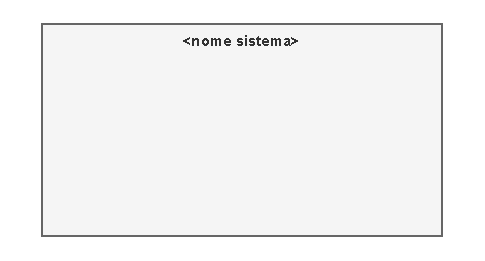
\includegraphics{Sezioni/ProcessiPrimari/Immagini/sistema_caso_uso.pdf}
        \caption{Rappresentazione del sistema in UML.}
        \label{fig:sistema_uml}
    \end{figure}
    
    \item \textbf{Attori}: rappresentano soggetti che interagiscono con il sistema software. Gli attori possono essere persone, altri applicativi o dispositivi che utilizzano le funzionalità del sistema.
    Un attore viene rappresentato nei diagrammi usando una delle due notazioni mostrate in \hyperref[fig:attori_uml]{Figura \ref{fig:attori_uml}} posta al di fuori del sistema.
    \begin{figure}[H]
        \centering
        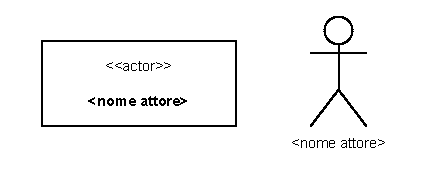
\includegraphics{Sezioni/ProcessiPrimari/Immagini/attori_caso_uso.pdf}
        \caption{Rappresentazione degli attori in UML.}
        \label{fig:attori_uml}
    \end{figure}
    
    \item \textbf{Casi d'uso}: rappresentano le funzionalità o i servizi offerti dal sistema che producono un risultato di valore per un attore. Ogni caso d'uso descrive una sequenza specifica di interazioni tra gli attori e il sistema.
    Ogni caso d'uso viene rappresentato nei diagrammi usando la notazione mostrata in \hyperref[fig:caso_uso]{Figura \ref{fig:caso_uso}} posta all'interno del sistema.
    \begin{figure}[H]
        \centering
        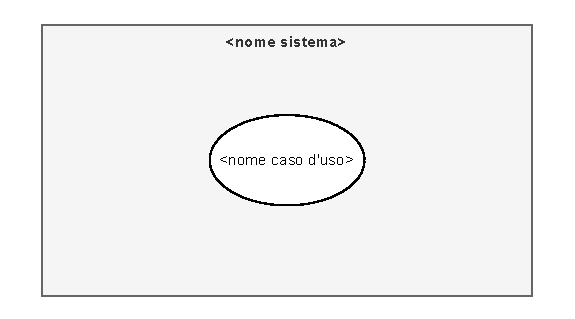
\includegraphics{Sezioni/ProcessiPrimari/Immagini/caso_uso.pdf}
        \caption{Rappresentazione caso d'uso in UML.}
        \label{fig:caso_uso}
    \end{figure}
    
    \item \textbf{Relazioni}.
    
    Sono delle notazioni che permettono di rendere più modulari i diagrammi di casi d'uso e di rendere chiara l'interazione degli attori con il sistema.
    
    \begin{itemize}
        \item \textbf{Associazione}: è la relazione fondamentale che collega un attore a un caso d'uso a cui esso partecipa.
        Uno stesso attore può partecipare a \texttt{N} casi d'uso.
        Le associazioni vengono rappresentate in UML come mostrato in \hyperref[fig:associazione_uml]{Figura \ref{fig:associazione_uml}}.
        \begin{figure}[H]
            \centering
            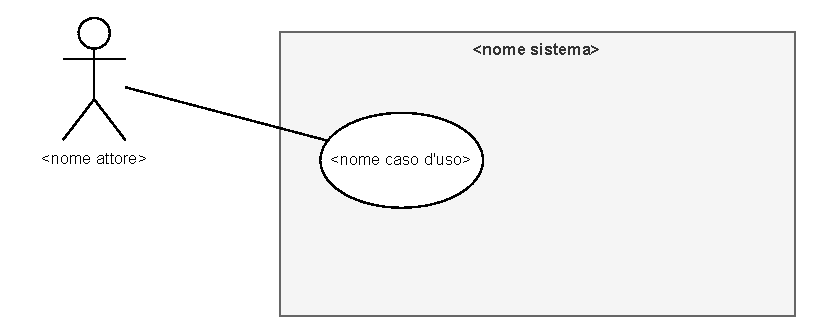
\includegraphics{Sezioni/ProcessiPrimari/Immagini/associazione_uml.pdf}
            \caption{Rappresentazione associazione in UML.}
            \label{fig:associazione_uml}
        \end{figure}

        \item \textbf{Inclusione}: rappresenta una dipendenza in cui il comportamento del caso d'uso incluso è incorporato ogni volta che viene eseguito il caso d'uso base. Il caso d'uso incluso contiene funzionalità che sono riutilizzate in più casi d'uso principali, permettendo di evitare la duplicazione di comportamenti comuni.
        L'inclusione viene rappresentata in UML come mostrato in \hyperref[fig:inclusione_uml]{Figura \ref{fig:inclusione_uml}}.
        \begin{figure}[H]
            \centering
            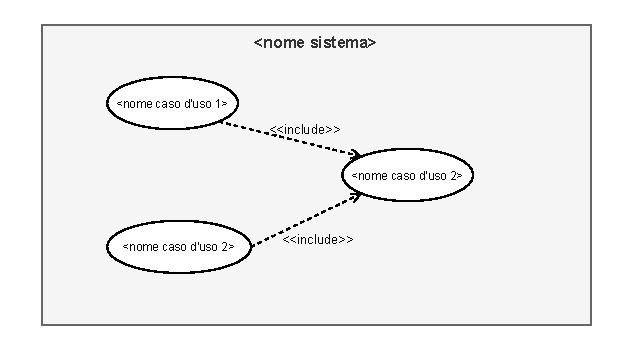
\includegraphics{Sezioni/ProcessiPrimari/Immagini/inclusione_uml.pdf}
            \caption{Rappresentazione inclusione in UML.}
            \label{fig:inclusione_uml}
        \end{figure}
        Come si può vedere nella \hyperref[tab:template_casi_uso]{Tabella \ref{tab:template_casi_uso}} è necessario:
        \begin{enumerate}
            \item Indicare il caso d'uso incluso come valore della colonna "Casi d'uso inclusi".
            \item Indicare lo step dello scenario principale o delle estensioni che utilizza il caso d'uso incluso.
            Questo viene fatto tramite la sintassi \texttt{include::<nome caso d'uso>}.
        \end{enumerate} 

        \item \textbf{Estensione}: mostra una relazione in cui un caso d'uso esteso aumenta le funzionalità del caso d'uso principale. Il caso d'uso esteso viene eseguito solo sotto determinate condizioni, interrompendo l'esecuzione del caso d'uso principale.
        L'estensione viene rappresentata in UML come mostrato in \hyperref[fig:estensione_uml]{Figura \ref{fig:estensione_uml}}.
        \begin{figure}[H]
            \centering
            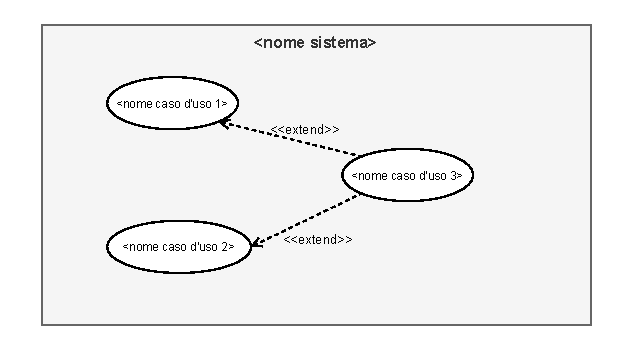
\includegraphics{Sezioni/ProcessiPrimari/Immagini/estensione_uml.pdf}
            \caption{Rappresentazione estensione in UML.}
            \label{fig:estensione_uml}
        \end{figure}
        
        \item \textbf{Generalizzazione}: rappresenta una relazione in cui un caso d'uso figlio può aggiungere funzionalità o modificare il comportamento di un caso d'uso genitore. Tutte le funzionalità definite nel caso d'uso genitore si mantengono nel caso d'uso figlio se queste non vengono ridefinite.
        La generalizzazione viene rappresentata in UML come mostrato in \hyperref[fig:generalizzazione_uml]{Figura \ref{fig:generalizzazione_uml}}.
        \begin{figure}[H]
            \centering
            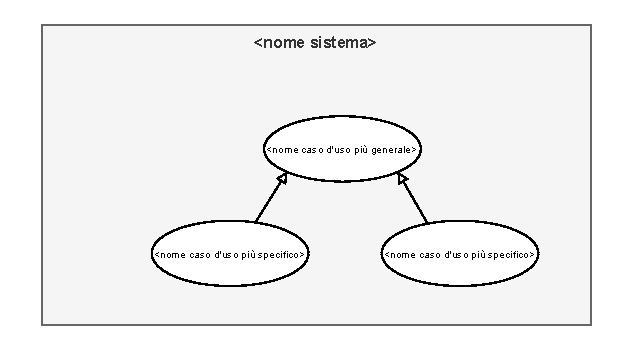
\includegraphics{Sezioni/ProcessiPrimari/Immagini/generalizzazione_uml.pdf}
            \caption{Rappresentazione generalizzazione in UML.}
            \label{fig:generalizzazione_uml}
        \end{figure}
        Come si può vedere nella \hyperref[tab:template_casi_uso]{Tabella \ref{tab:template_casi_uso}} è necessario indicare il caso d'uso genitore come valore della colonna "Caso d'uso base".

    \end{itemize}

    \item \textbf{Sottocasi d'uso}: i sottocasi d'uso rappresentano scenari specifici e dettagliati che si sviluppano all'interno di un caso d'uso principale. La loro funzione è di descrivere in modo approfondito le diverse situazioni o varianti operative che possono verificarsi nel contesto del caso d'uso generale.
    In particolare, ogni caso d'uso può essere suddiviso in più sottocasi, ciascuno associato a una specifica pagina o componente funzionale correlata al caso d'uso principale.
    
\end{itemize}

\paragraph{Fonti per l'Individuazione dei Casi d'Uso}
L'individuazione dei casi d'uso si basa principalmente sul capitolato fornito, che rappresenta una fonte essenziale per comprendere le caratteristiche generali del software da realizzare. 
Il capitolato, descrive le funzionalità principali e gli obiettivi del sistema, specificando alcuni requisiti chiave. 

Tuttavia, non tutti gli aspetti operativi sono dettagliati nel documento, il che rende necessaria un'integrazione attraverso deduzioni basate su necessità logiche e conoscenze pregresse. 
Il capitolato guida l'identificazione delle macro interazioni, consentendo di delineare i casi d'uso principali e il contesto generale in cui il sistema opererà. 
Tuttavia, nei punti in cui le specifiche risultano incomplete o generiche, è indispensabile adottare un approccio pro attivo, immaginando scenari d'uso che derivano dall'analisi delle esigenze tipiche di sistemi simili e delle best practices nel settore.

Questa attività di interpretazione si traduce nella definizione di ulteriori dettagli operativi, come eccezioni o varianti necessarie per garantire una piena copertura dei processi e un corretto funzionamento del sistema.

\subparagraph{Individuazione dei casi d'uso}
L'identificazione dei casi d'uso avviene attraverso i seguenti passaggi:
\begin{enumerate}
    \item \textbf{Identificazione degli attori}: Gli attori sono individuati in base ai loro ruoli e alle loro necessità operative. 
    Ad esempio, in un sistema gestionale possono essere individuati attori come l'amministratore, l'utente finale e un sistema di terze parti che si integra per la gestione dei pagamenti.
    L'identificazione degli attori è fondamentale per comprendere chi interagirà con il sistema e quali sono le operazioni che gli utenti devono poter eseguire.
    In \hyperref[fig:identificare_attori]{Figura \ref{fig:identificare_attori}} viene mostrata una tecnica utile per decidere se un concetto che appare nei requisiti è un attore o meno.
    \begin{figure}[H]
        \centering
        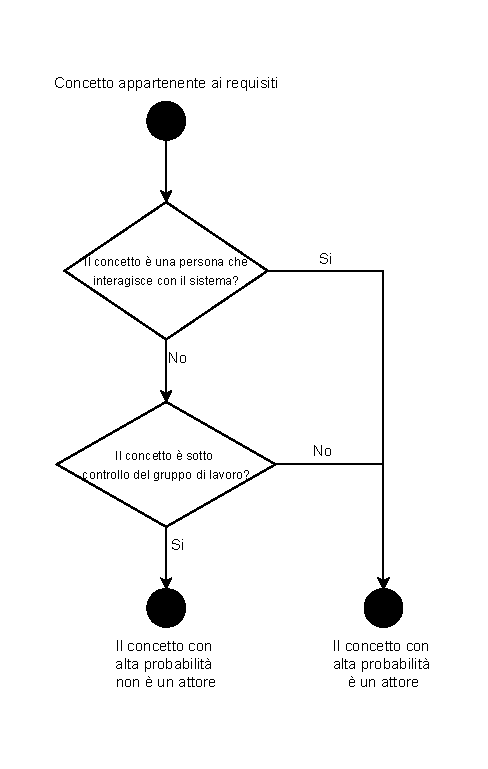
\includegraphics{Sezioni/ProcessiPrimari/Immagini/tecnica_casi_uso.pdf}
        \caption{Tecnica per identificare gli attori.}
        \label{fig:identificare_attori}
    \end{figure} 

    \item \textbf{Raffinamento attori}: Una coppia di attori può essere in una particolare relazione chiamata generalizzazione.
    In questa relazione l'attore "più generale" può eseguire un insieme di interazioni con il sistema che sono un sotto insieme delle interazioni che può eseguire l'attore "più specializzato".
    In altre parole l'attore "più specializzato" può eseguire tutte le interazioni che può eseguire l'attore "più generico" più eventuali ulteriori interazioni.
    In questo passaggio è importante scoprire queste relazioni tra gli attori.

    \item \textbf{Analisi degli obiettivi degli attori}: Una volta identificati gli attori e le relazioni tra essi, vengono analizzati i loro obiettivi in relazione al sistema. 
    Questo processo si basa sulla comprensione dei risultati che ogni attore desidera ottenere, come ad esempio la gestione di un ordine, l'accesso a report personalizzati o la possibilità di modificare parametri di configurazione.
    Gli obiettivi degli attori aiutano a delineare il perimetro dei casi d'uso e a definire le funzionalità che il sistema deve supportare per soddisfare tali obiettivi.

    \item \textbf{Identificazione dei casi d'uso principali}: Partendo dagli obiettivi individuati, si procede con la definizione dei casi d'uso principali. Questi rappresentano le macro funzionalità del sistema, cioè le interazioni essenziali e più frequenti tra gli attori e il sistema stesso. Ogni caso d'uso principale viene descritto in termini di azioni, e risultati attesi, garantendo che le funzionalità fondamentali siano chiaramente delineate.
    
    \item \textbf{Scomposizione in sotto-casi}: I casi d'uso principali possono venire successivamente scomposti in sotto-casi, se necessario, per dettagliare specifiche eccezioni, varianti o processi secondari. Questa scomposizione permette di descrivere scenari più specifici o complessi che possono verificarsi durante l'interazione. Ad esempio, il caso d'uso principale "Gestione di un ordine" può essere suddiviso nei sotto-casi "Modifica di un ordine esistente" e "Cancellazione di un ordine in attesa". Questo livello di dettaglio consente di rappresentare in modo accurato e completo tutti i comportamenti attesi del sistema.

\end{enumerate}

\section{Processi di supporto}
\label{sec:Processi_di_supporto}

\subsection{Documentazione}
\label{subsec:documentazione}
Il processo di documentazione ha lo scopo di registrare le informazioni prodotte da un processo primario garantendo la produzione di documenti coerenti e di qualità.

\subsubsection{Standard di formato}
I seguenti standard di formato sono validi per tutte le tipologie di documenti.
Questi standard devono sottostare agli standard specifici per ogni tipologia di documento indicata nel piano di documentazione.
Gli standard più specifici possono sovrascrivere i seguenti o specializzarli(es. data).

\paragraph{Standard di scrittura}
\begin{itemize}
    \item Le tabelle e le immagini devono preferibilmente comparire nella posizione in cui sono specificate all'interno del codice sorgente.
    \item Le tabelle e le immagini devono essere identificate da una label che deve essere usata ogni qual volta sia necessario farvi riferimento.
    \item Le tabelle e le immagini devono essere accompagnate da una caption che ne riassume il contenuto.
    \item Si devono utilizzare frasi non più lunghe di tre righe.
    \item I termini che appartengono al glossario devono essere indicati con una G a pedice e in corsivo.
    \item Si devono usare dei link per fare riferimento a elementi del documento.
\end{itemize}
Per informazioni pratiche sui punti sopra indicati leggere la sezione \hyperref[par:comandi_di_base]{Comandi di base}.

\paragraph{Standard di forma}

\subparagraph{Intestazione}
Ogni pagina deve contenere nell'intestazione le seguenti informazioni:
\begin{lstlisting}
    Nome documento - <versione>
\end{lstlisting}
Dove la versione rispetta le regole indicate alla sezione \hyperref[par:versione_documenti]{Versione dei documenti}. 

\subparagraph{Prima pagina}
La prima pagina deve contenere le seguenti informazioni:
\begin{itemize}
    \item Nome documento.     
    \item Nome gruppo.
    \item Data. 
    \item Versione.
    \item Logo del gruppo.
\end{itemize}

\subparagraph{Seconda pagina}
La seconda pagina deve contenere il registro delle modifiche per ogni file sottoposto a controllo di configurazione.
Il contenuto e la gestione del registro è indicato alla sezione \hyperref[par:registro_delle_modifiche]{Registro delle modifiche}.

\subparagraph{Terza pagina}
La terza pagina deve contenere l'indice.

\subsubsection{Macro categorie di documenti}
Di seguito vengono elencate le due macro categorie di documenti. 

\paragraph{Documenti interni}
Servono al team di lavoro.
Sono:
\begin{itemize}
    \item Verbali interni.
    \item Norme di progetto.
\end{itemize}

\paragraph{Documenti esterni}
Servono al team di lavoro e alla proponente.
Sono:
\begin{itemize}
    \item Piano di progetto.
    \item Verbali esterni.
    \item Analisi dei requisiti.
    \item Piano di qualifica.
\end{itemize}

\subsubsection{Piano di documentazione}
Di seguito viene riportato il piano di documentazione in cui si definiscono le tipologie di documenti che verranno prodotti durante il ciclo di vita del prodotto e le loro caratteristiche.

\paragraph{Verbali interni}

\subparagraph{Scopo}
I verbali interni sono documenti che hanno lo scopo di registrare il prodotto di una riunione interna al team di lavoro.
Permettono quindi di avere una conoscenza condivisa delle decisioni prese e delle cose da fare.

\subparagraph{Autore}
L'autore dei verbali interni deve essere il Responsabile.

\subparagraph{Input}
Gli input per la stesura di questi documenti derivano direttamente dalla riunione interna eseguita solitamente a fine sprint ovvero ogni giovedì.

\subparagraph{Struttura}
I verbali interni sono composti dalle seguenti sezioni e sottosezioni:
\begin{enumerate}
    \item \textbf{Registro presenze}.
    
    Contiene le seguenti informazioni:
    \begin{enumerate}
        \item Data.
        \item Ora inizio.
        \item Ora fine.
        \item Piattaforma usata.
        \item Tabella che attesta la presenza dei membri del team.
        Intestazioni: Componente e Presenza.
    \end{enumerate}
    \item \textbf{Verbale}.
    \begin{enumerate}
        \item \textbf{Argomenti trattati}
        
        Contiene un riassunto dei temi trattati durante la riunione.
        Indica anche eventuali perplessità o difficoltà da introdurre nel diario di bordo.
        \item \textbf{Decisioni prese}.
        Contiene un riassunto delle decisioni prese durante la riunione indicando anche una giustificazione.
    \end{enumerate}

    \item \textbf{To Do}.
    
    Indica una lista delle cose da fare nel prossimo sprint collegandole alle informazioni di gestione della configurazione.
\end{enumerate}

\subparagraph{Standard di scrittura specifici}
\begin{itemize}
    \item La data del documento riguarda il giorno in cui è avvenuta la riunione interna.
\end{itemize}

\paragraph{Verbali esterni}

\subparagraph{Scopo}
I verbali esterni sono documenti che hanno lo scopo di registrare la conoscenza del team sulle necessità della proponente a seguito di una riunione esterna.
Permettono quindi la conferma di una conoscenza comune(team e proponente) sulle necessità che il prodotto colma.
Funzionano quindi da garanzia al team sul fatto che la sua direzione sia corretta.

\subparagraph{Autore}
L'autore dei verbali esterni deve essere il Responsabile.

\subparagraph{Input}
Gli input per la stesura di questi documenti derivano direttamente dalla riunione esterna che deve essere concordata in anticipo con la proponente.

\subparagraph{Struttura}
I verbali esterni sono composti dalle seguenti sezioni e sottosezioni:
\begin{enumerate}
    \item \textbf{Registro presenze}.
    
    Contiene le seguenti informazioni:
    \begin{enumerate}
        \item Data.
        \item Ora inizio.
        \item Ora fine.
        \item Piattaforma.
        \item Tabella che attesta la presenza dei membri del team.
        Intestazioni: Componente e Presenza.
        \item Tabella che attesta i rappresentati della proponente che hanno partecipato alla riunione.
        Intestazioni: Componente e Presenza.
    \end{enumerate}
    A fondo pagina viene lasciato spazio per permettere al proponente di firmare il verbale esterno.

    \item \textbf{Domande}.
    
    Lista delle domande esposte dal team.

    \item \textbf{Conclusioni}.
    
    Lista delle conclusioni che il team ha tratto dalle risposte date dai rappresentati della proponente.
\end{enumerate}

\subparagraph{Standard di scrittura specifici}
\begin{itemize}
    \item La data del documento riguarda il giorno in cui è avvenuta la riunione esterna.
\end{itemize}

\paragraph{Analisi dei requisiti}

\subparagraph{Scopo}
Questo documento ha lo scopo di racchiudere i requisiti utente e i requisiti software sul prodotto oggetto del capitolato.

\subparagraph{Autore}
Gli autori di questo documento sono gli Analisti.

\subparagraph{Input}
Gli input per la stesura del documento di analisi dei requisiti derivano dall'attività di analisi dei requisiti.

\subparagraph{Struttura}
La struttura del documento di analisi dei requisiti è composta dalle seguenti sezioni:
\begin{enumerate}
    \item \textbf{Descrizione prodotto}.
    
    Ha lo scopo di descrivere il sistema a un alto livello di astrazione.
    Questa sezione è composta dalle seguenti sottosezioni:
    \begin{enumerate}
        \item \textbf{Obiettivi prodotto}.
        
        Descrive il bisogno che ha portato alla stesura del capitolato e come il prodotto le soddisfa.
        
        \item \textbf{Funzioni prodotto}.

        Descrive le funzioni principali del prodotto.

        \item \textbf{Caratteristiche utente}.
        
        Descrive gli utenti che useranno il sistema e le loro caratteristiche.
    \end{enumerate}

    \item \textbf{Use case}.
    
    Descrive i requisiti utente e l'analisi che porta ai requisiti software.
    

    \item \textbf{Requisiti funzionali di qualità e di vincolo}.
    
    Elenca i requisiti funzionali e non.
    
\end{enumerate}

\paragraph{Norme di progetto}
Il presente documento ha lo scopo indicato nell'introduzione.

\subparagraph{Autore} 
L'autore di questo documento è l'Amministratore.

\subparagraph{Input}
Gli input per la stesura del documento delle norme di progetto derivano dal processo di gestione.

\subparagraph{Struttura}
Deve esistere una sezione per ogni categoria di processo e una sottosezione per ogni processo indicato nello standard IEEE 12207:1996 usato dal team.

\paragraph{Piano di progetto}
Il documento piano di progetto contiene le informazioni che permettono la gestione di progetto da parte del Responsabile.

\subparagraph{Autore} 
L’autore di questo documento è il Responsabile.

\subparagraph{Input}
Gli input per la stesura del documento delle norme di progetto derivano dal processo di gestione.

\subparagraph{Struttura}
\label{subsec:struttura_piano}
Il piano di progetto è composto dalle seguenti sezioni:
\begin{enumerate}
    \item \textbf{Analisi dei rischi}.
    
    Contiene l'output dell'attività di analisi dei rischi.

    \item \textbf{Stima dei costi}.
    
    Contiene la stima delle ore che il gruppo ritiene di consumare e i costi che derivano dalle stesse. 
    
    \item \textbf{Milestone principali}.
    
    Definisce le milestone principali che devono essere sottoposte alla validazione del proponente e/o del committente.
    Per ogni milestone vengono indicate:
    \begin{itemize}
        \item Data di consegna.
        \item Baseline.
        \item Risorse preventivate.
    \end{itemize}
    
    \item \textbf{Primo periodo}.
    
    Indica l'insieme di risorse utilizzate nel primo periodo di progetto durante il quale la pianificazione era ancora confusionaria.
    
    Viene quindi mostrato lo stato delle risorse col termine del primo periodo nelle sottosezioni:
    \begin{enumerate}
        \item \textbf{Consuntivo}.
        
        Tabella composta dalle colonne: "Ruolo", "Ore consumate".

        \item \textbf{Aggiornamento rimaste}.
        
        Tabella composta dalle colonne: "Ruolo", "Ore rimaste".
    \end{enumerate}
    
    \item \textbf{Sprint}
    
    Per ogni sprint contiene una sottosezione chiamata \texttt{sprint n} che a sua volta contiene le seguenti sottosezioni:
    \begin{enumerate}
        \item \textbf{Obbiettivi}.
        
        Descrizione degli obbiettivi dello sprint tramite una lista puntata contenente la descrizione di essi e le issue assegnate a ogni obbiettivo.
        \item \textbf{Pianificazione}.
        
        Tabella composta dalle colonne: "Identificativo richiesta di modifica", "Ore preventivate" e "Ruolo".

        \item \textbf{Consuntivo}.
        
        Tabella composta dalle colonne: "Identificativo richiesta di modifica", "Ore sviluppo", "Ore verifica" e "Stato".
        Dove "Stato" viene indicato seguendo la convenzione \hyperref[par:stati]{Stati delle richieste di modifica}.
        
        \item \textbf{Retrospettiva}.
        
        Descrizione dei problemi e dei rischi verificati durante lo sprint.

        \item \textbf{Aggiornamento risorse rimaste}.
        
        Aggiornamento delle risorse restanti in seguito allo sprint tramite la tabella:
        "Ruolo", "Ore rimanenti".
        
    \end{enumerate}

\end{enumerate}

\subsection{Gestione della configurazione}
\label{subsec:gestione_della_configurazione}
Il processo di gestione della configurazione si occupa di applicare procedure amministrative e tecniche durante tutto il ciclo di vita del software. 
In particolare identifica e definisce gli elementi software di un sistema per tenere traccia: delle modifiche, dello stato e dei rilasci dei file.
Inoltre garantisce la completezza, la coerenza e la correttezza degli elementi che compongono il prodotto software.

\subsubsection{Repository}
\label{subsubsec:repository}
I prodotti del progetto vengono memorizzati in più \glossario{repository}.
Di seguito vengono elencati i repository utilizzati dal gruppo, le loro caratteristiche e la loro struttura.

\paragraph{SorgentiDocumentazione}
Questo repository contiene i sorgenti della documentazione scritti usando il \hyperref[par:latex]{linguaggio LaTeX}.
Il repository segue la struttura indicata in \hyperref[fig:repo_sorgenti_documenti]{Figura \ref{fig:repo_sorgenti_documenti}}.
\begin{figure}[H]
    \dirtree{%
        .1 SorgentiDocumentazione.
            .2 .github.
                .3 DizionariLatex.
                    .4 \texttt{<dizionari>}.
                .3 workflows.
                    .4 \texttt{<file workflows>}.
            .2 Candidatura.
            .2 RTB.
            .2 Packages.
            .2 Immagini.
            .2 \texttt{README.md}.
            .2 \texttt{.gitignore}.
    }
    \caption{Struttura repository SorgentiDocumentazione.}
    \label{fig:repo_sorgenti_documenti}
\end{figure}
Dove:
\begin{enumerate}
    \item \texttt{Candidatura}, \texttt{RTB} e \texttt{Packages} sono delle cartelle il cui contenuto viene spiegato nelle successive sezioni.
    \item \texttt{<file workflows>} sono dei file che definiscono le automazioni associate al repository e vengono denominati usando la sintassi \glossario{Pascal case}.
    \item \texttt{Immagini} è una cartella che contiene il logo del gruppo.
    \item \texttt{README.md} è un file che contiene la descrizione del repository e del gruppo.
    \item \texttt{.gitignore} è un file speciale che contiene una lista di file che il sistema di versionamento deve ignorare.
\end{enumerate}

\subparagraph{Candidatura}
La cartella candidatura ha la struttura indicata in \hyperref[fig:repo_sorgenti_documenti_candidatura]{Figura \ref{fig:repo_sorgenti_documenti_candidatura}}.
\begin{figure}[H]
    \dirtree{%
        .1 Candidatura.
            .2 VerbaliEsterni.
                .3 \texttt{<verbali esterni esplicativi>}.
            .2 VerbaliInterni.
                .3 \texttt{<verbali interni>}.
            .2 \texttt{<lettera di candidatura>}.
            .2 \texttt{<preventivo dei costi assunzione impegni>}.
            .2 \texttt{<valutazione capitolati>}.
    }
    \caption{Struttura cartella Candidatura.}
    \label{fig:repo_sorgenti_documenti_candidatura}
\end{figure}

\subparagraph{RTB}
La cartella RTB ha la struttura indicata in \hyperref[fig:repo_sorgenti_documenti_RTB]{Figura \ref{fig:repo_sorgenti_documenti_RTB}}.
\begin{figure}[H]
    \dirtree{%
        .1 RTB.
            .2 DocumentiInterni.
                .3 \texttt{<norme di progetto>}.
                .3 VerbaliInterni.
                .4 \texttt{<verbali interni>}.
            .2 DocumentiEsterni.
                .3 \texttt{<piano di progetto>}.
                .3 \texttt{<analisi dei requisiti>}.
                .3 VerbaliEsterni.
                    .4 \texttt{<verbali esterni>}.
    }
    \caption{Struttura cartella RTB.}
    \label{fig:repo_sorgenti_documenti_RTB}
\end{figure}

\subsubsection{Identificazione configuration item}
\label{subsubsec:identificazione_CI}
Di seguito vengono elencate le regole usate per nominare i \glossario{configuration item} elencati nella sezione \hyperref[subsubsec:repository]{repository}.
I file che non riguardano direttamente il progetto non vengono spiegati ulteriormente. 

\paragraph{Sorgenti documenti}
\begin{table}[H]
    \resizebox{\textwidth}{!}{
    \begin{tabular}{| c | c | c |}
        \hline
        \textbf{Nome} & \textbf{Identificativo} & \textbf{Registro modifiche} \\
        \hline 
        verbali interni & \texttt{<data>-<versione>} & sì \\
        \hline
        verbali esterni & \texttt{<data>-<versione>} & sì\\
        \hline
        verbali esterni esplicativi & \texttt{<data>-<proponente>-<versione>} & sì\\
        \hline
        lettera di candidatura & \texttt{LetteraDiCandidatura} & no\\
        \hline
        valutazione dei capitolati & \texttt{ValutazioneDeiCapitolati-<versione>} & sì\\
        \hline
        preventivo dei costi e assunzione impegni & \texttt{CostiImpegni-<versione>} & sì\\
        \hline
        piano di progetto & \texttt{PianoDiProgetto-<versione>} & sì\\
        \hline
        norme di progetto & \texttt{NormeDiProgetto-<versione>} & sì\\
        \hline
        Piano di qualifica & \texttt{PianoDiQualifica-<versione>} & sì\\
        \hline
        analisi dei requisiti & \texttt{AnalisiDeiRequisiti-<versione>} & sì\\
        \hline
    \end{tabular}}
    \caption{Configuration item del repository SorgentiDocumentazione.}
\end{table}
\noindent Dove:
\begin{itemize}
    \item Le date seguono lo schema \texttt{aaaa\_mm\_gg}.
    \item Il nome della proponente segue la sintassi \glossario{Pascal case}.
    \item Le versioni seguono lo schema indicato alla sezione \hyperref[par:versione_documenti]{Versione dei documenti}.
\end{itemize}
Il motivo dell'utilizzo di data e proponente all'interno dei nomi di alcune tipologie di documenti è che permettono un ordinamento sensato degli stessi.

\subsubsection{Controllo di versione}
Di seguito vengono riportati i metodi usati dal gruppo per tenere traccia delle versioni dei file contenuti nei repository.

\paragraph{Software di controllo di versione}
Il gruppo ha deciso di utilizzare Git come software per il controllo di versione.
I motivi di questa scelta sono:
\begin{enumerate}
    \item Git è abbastanza conosciuto dai membri del gruppo.
    \item Git è molto usato e quindi una conoscenza approfondita dello stesso è molto utile.
\end{enumerate}
Di seguito vengono fornite delle informazioni teoriche sulle scelte fatte dal gruppo sulla gestione del repository.
La separazione netta tra concetti teorici e pratici pur essendo "fastidiosa" per il lettore permette la modularità degli strumenti usati.

\subparagraph{Strategia di branching}
\label{subpar:strategia_di_branching_documenti}
Come \glossario{strategia di branching} il gruppo ha scelto l'utilizzo di Gitflow dato che permette di massimizzare il lavoro parallelo riducendo la complessità di risoluzione dei conflitti.
In \hyperref[fig:gitflow]{Figura \ref{fig:gitflow}} viene mostrato un esempio di utilizzo della strategia di branching Gitflow.
\begin{figure}[H]
    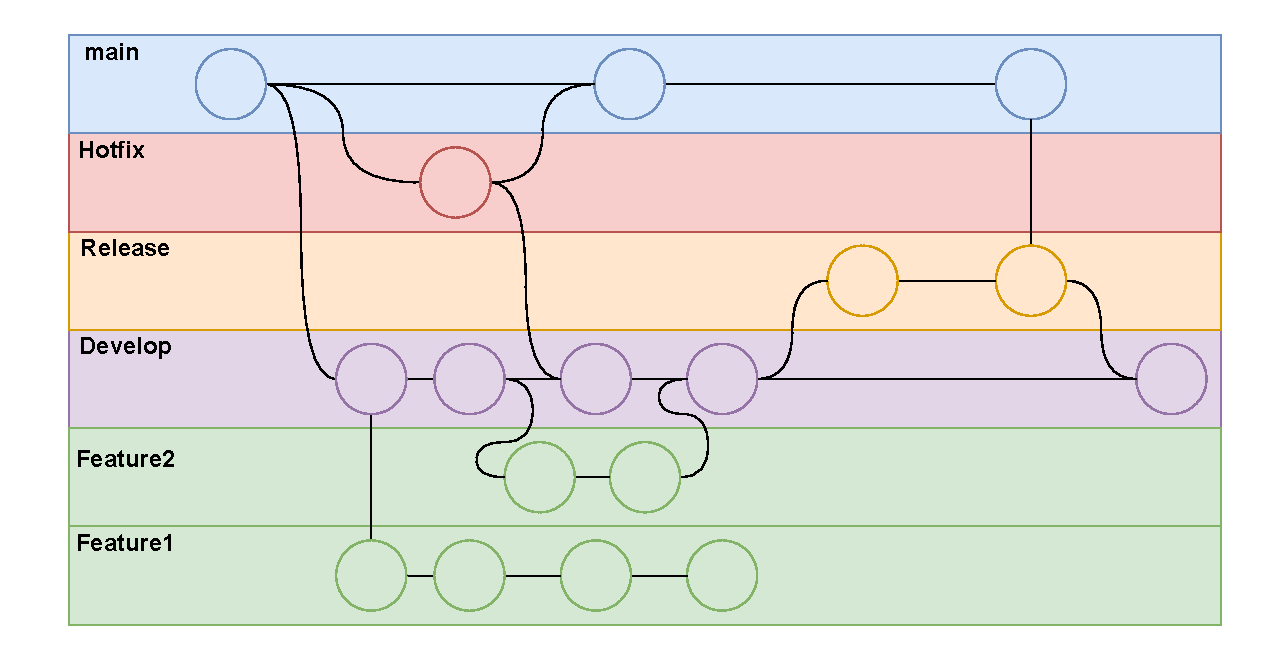
\includegraphics[scale=0.65]{Sezioni/ProcessiDiSupporto/Immagini/gitflow.pdf}
    \caption{Gitflow in azione(i cerchi sono commit e le linee i collegamenti tra essi)}
    \label{fig:gitflow}
\end{figure}
Di seguito vengono descritti i rami utilizzati da Gitflow e le convenzioni usate dal gruppo.
\begin{enumerate}

\item \textbf{main}

Il ramo \texttt{main} contiene la codeline principale ovvero le versioni dei file che compongono l'ultima baseline raggiunta.
Questo ramo è un ramo "stabile" nel senso che persiste nel repository lungo tutta la sua vita.

\item \textbf{develop}

Il ramo \texttt{develop} contiene la codeline secondaria ovvero i cambiamenti verificati che si sommeranno formando la prossima baseline.
Anche questo ramo è un ramo "stabile" e viene creato a partire dal ramo \texttt{main}.

\item \textbf{feature}
\label{item:rami_feature}
I rami \texttt{feature} vengono usati dai membri del gruppo per implementare le modifiche.
Sono dei rami "provvisori" nel senso che esistono finché il loro contenuto non viene verificato.
I rami \texttt{feature} vengono creati a partire dal ramo \texttt{develop} e confluiscono in esso quando il loro contenuto passa con successo la verifica.
Il gruppo ha deciso di utilizzare la seguente convenzione per la denominazione di questi rami:
\begin{lstlisting}
    feature/#<idRichiestaDiModifica>
\end{lstlisting}
Così facendo si ottiene un collegamento immediato tra ramo di \texttt{feature} e richiesta di modifica.

\item \textbf{hotfix}

I rami \texttt{hotfix} vengono usati per eseguire modifiche rapide e di dimensioni ridotte.
Queste modifiche non influenzano quindi le versioni dei documenti.
Questi rami sono "provvisori" nel senso che vengono eliminati dopo che le loro modifiche sono state allineate ai rami \texttt{main} e \texttt{develop}.


\item \textbf{release}

I rami \texttt{release} vengono usati dal Responsabile del gruppo per approvare il contenuto del ramo \texttt{develop} consolidandolo in una baseline nella codeline principale.
Sono dei rami "provvisori" nel senso che esistono finché il loro contenuto non viene approvato.
I rami \texttt{release} vengono creati a partire dal ramo \texttt{develop} e confluiscono nei rami \texttt{main} e \texttt{develop}.
Il gruppo ha deciso di utilizzare la seguente convenzione per la denominazione di questi rami:
\begin{lstlisting}
    feature/nomeMilestone
\end{lstlisting}
Così facendo si ottiene un collegamento immediato tra ramo di \texttt{release} e la milestone che raggiunge.
\end{enumerate}

\subparagraph{Risoluzione dei conflitti}
\label{subpar:risoluzione_dei_conflitti}
Utilizzando Gitflow i conflitti possono presentarsi nelle seguenti fusioni(merge) di rami(indicate come "partenza \textrightarrow\ destinazione"):
\begin{enumerate}
    \item \textbf{release} \textrightarrow\ \textbf{main}
    
    I conflitti si presentano quando nel ramo di \texttt{release} esistono modifiche su uno o più file presenti nel ramo \texttt{main}.
    In questo caso il contenuto del ramo \texttt{release} ha la precedenza dato che è più aggiornato.
    
    \item \textbf{hotfix} \textrightarrow\ \textbf{develop}
    
    I conflitti si presentano quando la correzione rapida eseguita nel ramo \texttt{hotfix} riguarda uno o più file che nel mentre sono stati modificati nel ramo \texttt{develop}.
    In questo caso è importante che le correzioni del ramo \texttt{hotfix} persistano nel ramo \texttt{develop} dopo la fusione.
    Il ramo \texttt{hotfix} ha quindi la precedenza.   


    \item \textbf{feature} \textrightarrow\ \textbf{develop}
   
    I conflitti possono presentarsi se due membri del gruppo lavorano sullo stesso documento allo stesso tempo.
    In questo caso entrambe le modifiche verificate devono raggiungere il ramo \texttt{develop}.
    Bisogna però porre attenzione a mantenere il corretto ordine del \hyperref[par:registro_delle_modifiche]{Registro delle modifiche}.
\end{enumerate}


\paragraph{Registro delle modifiche}
\label{par:registro_delle_modifiche}
Oltre all'utilizzo di un software di controllo di versione il gruppo ha deciso di dotare alcuni documenti di una tabella chiamata registro delle modifiche.
Tale tabella se il repository fosse gestito in modo impeccabile sarebbe una copia dei dati già registrati nella stessa.
Tuttavia il metodo di lavoro del gruppo è in continua evoluzione quindi possono accadere modifiche distruttive che eliminano le versioni dei configuration item apparteneti alla baseline precedente.
Il registro delle modifiche è quindi uno strumento a supporto del controllo di configurazione ed è più "attendibile" rispetto alla storia del repository Git.
I documenti per cui viene usato il registro delle modifiche sono indicati nella sezione \hyperref[subsubsec:identificazione_CI]{Identificazione configuration item}.

Di seguito viene indicata la struttura del registro delle modifiche:
\begin{enumerate}
    \item \textbf{Versione}: versione del documento dopo la verifica della modifica.
    \item \textbf{Data}: data in cui è avvenuta la modifica.
    \item \textbf{Autore/i}: nome e cognome dei componenti del gruppo che hanno eseguito le modifiche.
    \item \textbf{Verificatore/i}: nome e cognome dei verificatori.
    \item \textbf{Descrizione}: breve descrizione delle modifiche indicando un link alle sezioni modificate.
    
    La descrizione permette ai membri del team di capire velocemente la necessità di allinearsi a nuove informazioni. 
\end{enumerate} 
\textbf{Nota bene}: Le righe del registro delle modifiche sono ordinate per versione decrescente.

\paragraph{Versione}
\label{par:versione_documenti}
Le versioni dei documenti vengono indicate seguendo lo schema di versionamento:
\begin{lstlisting}
    vX.Y
\end{lstlisting}
Dove:
\begin{enumerate}
    \item \texttt{X}: intero positivo che indica la versione major del documento.
    La versione major indica a quante volte il documento ha raggiunto uno stato ritenuto come "stabile" dal gruppo.

    \item \texttt{Y}: intero positivo che indica la versione minor del documento.
    La versione minor indica il numero di modifiche effettuate al documento a seguito dell'ultima versione major.
\end{enumerate}
Uno schema di versionamento a due valori risulta più semplice dato che si concentra solo sulle modifiche significative in termini di contenuto dei documenti.

\textbf{Nota bene}: per evitare ambiguità con le estensioni dei documenti il gruppo ha deciso di rappresentare la versione nei nomi dei documenti usando la notazione \texttt{vX\_Y}.

\subsubsection{Gestione delle modifiche}
Una modifica è intesa come un azione che ha lo scopo di modificare lo stato di uno o più file appartenenti all'ultima baseline raggiunta in un repository. 

\paragraph{Richieste di modifica}
Ogni modifica deve essere preceduta da una richiesta di modifica che deve essere discussa e accettata tramite votazione di maggioranza.
Le richieste di modifica vengono registrate e gestite utilizzando il servizio di issue tracking offerto da GitHub.  
Le informazioni tecniche riguardanti la gestione delle issue vengono indicate alla sezione \hyperref[subpar:ITS]{Issue Tracking System}.
Una richiesta di modifica deve contenere le seguenti informazioni:
\begin{itemize}
    \item \textbf{Nome del file da modificare}: indicandone il percorso all'interno del repository.
    \item \textbf{Data della richiesta}.
    \item \textbf{Tempo stimato per implementare il cambiamento}: indicata nel piano di progetto nella pianificazione dello sprint attuale.
    \item \textbf{Tipo di modifica}.
    \item \textbf{Descrizione della modifica da fare}.
    \item \textbf{Stato}: indica lo stato della richiesta al momento e permette al gruppo di capire cosa fare.
\end{itemize}

\subparagraph{Descrizione modifica}
La descrizione di una modifica deve essere rappresentata tramite un check list contenente i compiti da svolgere per implementare la modifica.
Questo permette:
\begin{enumerate}
    \item [a.] A chi implementa la modifica di avere una linea guida su cosa fare anche dopo tanto tempo rispetto alla discussione della modifica nel gruppo.
    \item [b.] A chi verifica la modifica di sapere che cosa doveva essere fatto.
\end{enumerate} 

\paragraph{Ciclo di vita delle richieste di modifica}
\label{par:ciclo_vita_richieste_di_modifica}
Gli stati che una richiesta di modifica attraversa durante il suo ciclo di vita sono riassunti nel diagramma in \hyperref[fig:ciclo_di_vita_modifiche_documenti]{Figura \ref{fig:ciclo_di_vita_modifiche_documenti}}.
\begin{figure}[h!]
    \center
    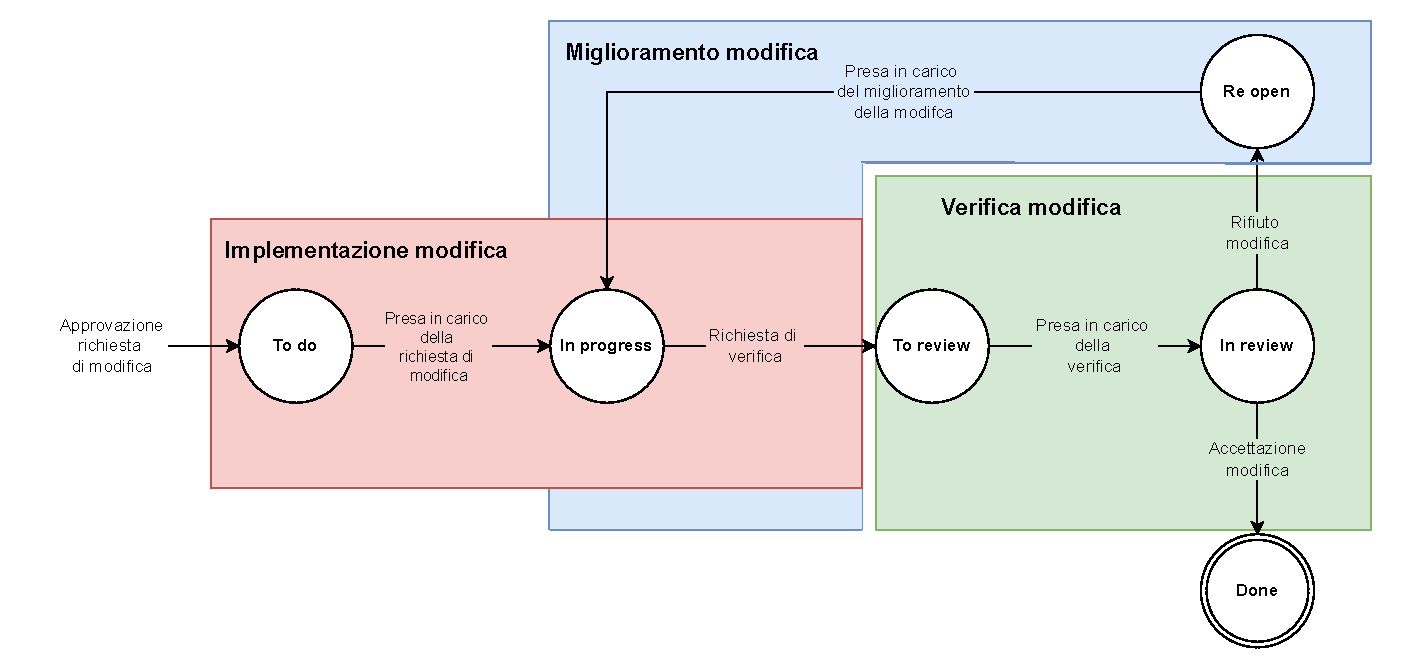
\includegraphics[scale=0.6]{Sezioni/ProcessiDiSupporto/Immagini/lifecycle_modifica.pdf}
    \caption{Ciclo di vita di una richiesta di modifica}
    \label{fig:ciclo_di_vita_modifiche_documenti}
\end{figure}

\paragraph{Stati}\label{par:stati}
In particolare gli stati di una richiesta di modifica sono:
\begin{enumerate}
    \item \textbf{To do}: la richiesta di modifica è stata approvata dal gruppo, registrata in GitHub e appartiene ai compiti che portano al raggiungimento di una prossima baseline.
    \item \textbf{In progress}: la richiesta di modifica è stata presa in carico da un membro del gruppo.
    \item \textbf{To review}: la modifica è stata implementata dal membro del gruppo che la presa in carico.
    Prima di contribuire alla prossima baseline deve essere verificata.
    \item \textbf{In review}: un Verificatore sta procedendo a eseguire la verifica della modifica.
    \item \textbf{Re open}: la modifica non è stata accettata dal Verificatore e deve quindi essere migliorata.
    \item \textbf{Done}: la modifica è stata accettata dal Verificatore e quindi è stata integrata nella prossima baseline. 
\end{enumerate}

\paragraph{Cambiamenti di stato}
I cambiamenti di stato di una richiesta di modifica durante al suo ciclo di vita sono:
\begin{enumerate}
    \item \textbf{Presa in carico della richiesta di modifica}(\textbf{To do} \textrightarrow\ \textbf{In progress})
    
    Avviene manualmente seguendo la procedura a carico del modificatore indicata alla sezione \hyperref[subpar:presa_carico_modifica]{Presa in carico di una modifica}.
    
    \item \textbf{Richiesta di verifica}(\textbf{In progress} \textrightarrow\ \textbf{To review})
    
    Avviene manualmente seguendo la procedura a carico del modificatore indicata alla sezione \hyperref[subpar:github_richiesta_di_verifica]{Richiesta di verifica}.
    
    \item \textbf{Presa in carico della verifica}(\textbf{To review} \textrightarrow\ \textbf{In review})
    
    Avviene manualmente seguendo la procedura indicata alla sezione \hyperref[subpar:presa_carico_verifica]{Presa in carico di una verifica}.
    
    \item  \textbf{Rifiuto modifica}(\textbf{In review} \textrightarrow\ \textbf{Re open})
    
    Avviene in automatico nel caso in cui la verifica della modifica abbia esito negativo.
    
    \item \textbf{Accettazione modifica}(\textbf{In review} \textrightarrow\ \textbf{Done})
    
    Avviene in automatico nel caso in cui la verifica della modifica abbia esito positivo.
    
    \item \textbf{Presa in carcio del migliroamento della modifica}(\textbf{Re open} \textrightarrow\ \textbf{In progress})
    
    Avviene manualmente seguendo la procedura a carico del modificatore indicata alla sezione \hyperref[subpar:presa_carico_modifica]{Presa in carico di una modifica}.
\end{enumerate}

\paragraph{Fasi}
Le fasi del ciclo di vita di una modifica sono:
\begin{enumerate}
    \item \textbf{Implementazione modifica}: comprende gli stati "To do", "In progress", "To review" e le transizioni tra gli stessi.

    \item \textbf{Verifica modifica}: comprende gli stati "To review", "In review", "Done", "Re open" e le transizioni tra gli stessi.
    
  
    \item \textbf{Miglioramento modifica}: comprende gli stati "Re open", "In progress", "To review" e le transizioni tra gli stessi. 
  
\end{enumerate}

\subparagraph{Implementazione modifica}
Per implementare una modifica è necessario eseguire i seguenti passi:
\begin{enumerate}
\item \hyperref[subpar:presa_carico_modifica]{Presa in carico della modifica}.

\item \hyperref[subpar:pull]{Pull ramo} \texttt{develop}.

\item \hyperref[subpar:branch]{Creazione ramo} \texttt{feature}(vedere \hyperref[item:rami_feature]{rami feature}).

\item Colmare la necessità della richiesta di cambiamento assicurandosi di soddisfare la check list.
Questa operazione deve avvenire seguendo il processo che regola l'implementazione della tipologia di file da modificare.

\textbf{Nota bene}: Per alcuni documenti è necessario aggiungere al \hyperref[par:registro_delle_modifiche]{registro delle modifiche} una nuova riga contenente le informazioni per le colonne "Autore/i" e "Descrizione". 

\item \hyperref[subpar:commit]{Commit} delle modifiche nel ramo \texttt{feature}.

\item \hyperref[subpar:push]{Push ramo} \texttt{feature}.

\item \hyperref[subpar:github_richiesta_di_verifica]{Richiesta di verifica} aggiungendo nel primo commento della
 pull request i seguenti campi:
 \begin{enumerate}
    \item closes \#\textless ID della issue che richiede la verifica\textgreater
    \item Tempo impiegato: \textless numero delle ore effettive usate per svolgere la issue\textgreater
 \end{enumerate}

\end{enumerate}

\subparagraph{Verifica modifica}
Per verificare un cambiamento è necessario eseguire i seguenti passi:
\begin{enumerate}
    \item \hyperref[subpar:presa_carico_verifica]{Presa in carico della verifica}.
    
    \item \hyperref[subpar:pull]{Pull} ramo \texttt{feature}(vedere \hyperref[item:rami_feature]{rami feature}).
    
    \item Verificare i cambiamenti seguendo le regole indicate nella sezione \hyperref[]{Verifica}.
    
    \textbf{Nota bene}: Nel caso di rifiuto per alcuni documenti è necessario aggiornare l'ultima riga del \hyperref[par:registro_delle_modifiche]{Registro delle modifiche} specificando la colonna "Verificatore/i".

    Nel caso di accettazione oltre a fare ciò è necessario specificare la colonna "Versione" e aggiornare la versione mostrata nel documento(leggere sezione \hyperref[par:struttura_di_base_documenti]{Struttura di base dei documenti}).

    \item \hyperref[subpar:commit]{Commit} delle modifiche sul ramo \texttt{feature}.
    
    \item \hyperref[subpar:push]{Push} del ramo \texttt{feature}.

    \item \hyperref[subpar:accettazione_modifiche]{Accettazione} o \hyperref[subpar:rifiuto_modifiche]{rifiuto} delle modifiche.
\end{enumerate}

\subparagraph{Miglioramento modifica}
  
Per eseguire il miglioramento di una modifica è necessario eseguire i seguenti passi:
\begin{enumerate}
\item \hyperref[subpar:presa_carico_modifica]{Presa in carico del miglioramento}.

\item \hyperref[subpar:pull]{Pull} branch \texttt{feature}(vedere \hyperref[item:rami_feature]{rami feature}).

\item Modificare il documento assicurandosi di soddisfare la check list e le informazioni aggiuntive date dal verificatore che ha rifiutato la modifica.
Questa operazione deve avvenire seguendo il processo che regola l'implementazione della tipologia di configuration item.

\textbf{Nota bene}: Per alcuni documenti è necessario aggiungere all'ultima riga del \hyperref[par:registro_delle_modifiche]{registro delle modifiche} le informazioni per la colonna "Autore/i". 

\item \hyperref[subpar:commit]{Commit} delle modifiche nel ramo \texttt{feature}.

\item \hyperref[subpar:push]{Push} ramo \texttt{feature}.

\item \hyperref[subpar:github_richiesta_di_verifica]{Richiesta di verifica}.
\end{enumerate}

\subsubsection{Approvazione}
Di seguito viene documentata l'attività di approvazione delle versioni dei file che devono essere consolidate in una baseline.
L'approvazione deve essere eseguita dal Responsabile del gruppo di lavoro e prevede le seguenti operazioni:
\begin{enumerate}
    \item Creazione ramo \texttt{release} seguendo le regole indicate nella sezione \hyperref[subpar:strategia_di_branching_documenti]{Strategia di branching}.
    \item Eseguire eventuali modifiche correttive minori.
    
    \textbf{Nota bene}: Aggiungere una nuova riga nel registro delle modifiche indicando i valori per le colonne "Autore/i", "Versione" e "Data".
    Inoltre usare il valore "Approvazione modifiche" per la colonna "Descrizione".

    \item \hyperref[subpar:commit]{Commit} delle modifiche.
    \item \hyperref[subpar:merge]{Merge} del ramo \texttt{release} nel ramo \texttt{main} e nel ramo \texttt{develop} seguendo le regole indicate alla sezione \hyperref[subpar:risoluzione_dei_conflitti]{Risoluzione dei conflitti}.
    \item \hyperref[subpar:push]{push} dei rami \texttt{main} e \texttt{develop}.
\end{enumerate}

\subsubsection{Distribuzione dei documenti}
La distribuzione dei documenti avviene mediante l'utilizzo di un sito web disponibile al link \href{https://alt-f4-eng.github.io/Documentazione/}{https://alt-f4-eng.github.io/Documentazione/}.
I documenti distribuiti vengono aggiornati ogni volta che viene modificata la baseline ovvero ogni volta che viene modificato il ramo \texttt{main}.
L'aggiornamento dei documenti segue la procedura indicata alla sezione \hyperref[par:pubblicazione_documenti]{Pubblicazione dei documenti}

\input{Sezioni/ProcessiDiSupporto/Sottosezioni/AccertamentoQualità.tex}

\subsection{Processo di Verifica}
\label{subsec:proc_verifica}
Il processo di verifica ha come obiettivo fondamentale l'accertamento che:
\begin{itemize}
    \item i \textbf{prodotti di lavoro} generati durante il \glossario{ciclo di vita} del software rispettino i requisiti specificati
    \item i \textbf{processi seguiti} siano conformi allo standard, alle linee guida e ai piani definiti
\end{itemize}
\subsubsection{Descrizione}
Questo processo consiste nel fornire prove oggettive che i risultati di una specifica fase dello sviluppo software rispettino tutti i requisiti previsti. 
Si basa sull’analisi e revisione del contenuto per valutare la coerenza, la completezza e la correttezza dei risultati. Nel caso di codice, include anche il testing per assicurarsi che i risultati siano conformi alle aspettative definite.
Le task fondamentali previste dal processo sono:
\begin{itemize}
    \item verifica dei processi;
    \item verifica dei requisiti;
    \item verifica della progettazione;
    \item verifica del codice;
    \item verifica della documentazione.
\end{itemize}
Per garantire l'accertamento della conformità, ogni volta che si apporta una modifica, è necessario sottoporre l'intero contenuto aggiornato a una verifica. 
L'incremento della versione del prodotto aggiornato avviene esclusivamente se la modifica viene verificata e la verifica ha esito positivo.
Il processo di verifica viene svolto dai membri incaricati come verificatori (che si segneranno all'interno del registro delle modifiche del documento). 
i quali non possono essere la stessa persona a cui è stata assegnata la realizzazione del prodotto da verificare.
\subsubsection{Analisi statica}
L'\glossario{analisi statica} è un approccio alla verifica che non richiede l'esecuzione del codice dell'oggetto di verifica per individuare i difetti del prodotto software 
e accertarne la sua completezza e coerenza.
Si applica non solo al codice, ma anche alla documentazione, verificando la conformità alle regole del prodotto, l'assenza di difetti e la presenza delle proprietà desiderate.
Dal team viene utilizzata una tecnica standard per l'\glossario{analisi statica} dei prodotti: \textbf{\glossario{Walkthrough}}.
\paragraph{Walkthrough}
Il \glossario{Walkthrough} è uno dei metodi di lettura nell'\glossario{analisi statica} utilizzato per esaminare e verificare una parte del prodotto, che sia documento o codice, per accertarne la conformità ai requisiti o vincoli stabiliti precedentemente.
Si tratta di un approccio collaborativo tra autore e verificatore durante il quale viene esaminato un prodotto o una sua parte, seguendo un percorso prestabilito e cercando di identificare difetti attraverso una lettura critica ad ampio spettro, priva di assunzioni.
Nel caso del controllo del codice, il verificatore deve simulare diverse possibili esecuzioni, mentre per i documenti deve analizzarne il contenuto.
Le fasi che vengono svolte durante questa tecnica di \glossario{analisi statica} sono:
\begin{itemize}
    \item \textbf{lettura}: il verificatore effettua una lettura critica dell'oggetto in esame cercando eventuali errori;
    \item \textbf{discussione}: al termine della lettura, nel caso vengano rilevati problemi, il verificatore comunica con gli autori e propone eventuali suggerimenti, con l'obiettivo di correggere i difetti;
    \item \textbf{correzione e repeat}: una volta terminata la discussione e rilevati i difetti, gli autori sono pregati di correggere tali difetti seguendo le indicazioni discusse. Successivamente, si passa di nuovo al passo 2.
\end{itemize}
\paragraph{verifica della documentazione}
La verifica della documentazione, composta solamente da \glossario{analisi statica} dei documenti realizzati e/o modificati, ha lo scopo di verificare
la qualità, completezza, coerenza e conformità dei documenti tecnici relativi al prodotto software da realizzare.
Durante l'esecuzione della tecnica di \glossario{Walkthrough} descritta precedentemente, il verificatore ha lo scopo di 
assicurarsi che vengano seguiti correttamente gli standard di scrittura e di forma, sia generici che specifici, indicati all'interno
del \hyperref[subsec:documentazione]{processo di Documentazione}.
Oltre a ciò, è stata realizzata una \glossario{GitHub Action} che, all'apertura di una \glossario{pull request}, realizza un'analisi grammaticale dei file 
modificati e coinvolti nella \glossario{pull request}, fornendo successivamente un \glossario{feedback} al gruppo di lavoro.
La \glossario{GitHub Action} assicura la correttezza grammaticale dei documenti verificati migliorando il processo di verifica, aumentandone l'efficienza 
e riducendo il tempo richiesto per le revisioni manuali, permettendo al verificatore di concentrarsi maggiormente su aspetti 
di forma e di contenuto.
\subsubsection{Analisi dinamica}
L'\glossario{analisi dinamica} è un approccio all'analisi di sitemi informatici e prodotti software che si concentra sull'osservazione e verifica
del loro comportamento durante l'esecuzione.
Quest'ultima è ampiamente impiegata per individuare errori a runtime, ottimizzare l'efficienza e testare la robustezza contro scenari imprevisti.
Grazie alla sua capacità di fornire dati concreti e rilevanti, rappresenta un elemento fondamentale nel processo di sviluppo e manutenzione di applicazioni e sistemi complessi.
Essa prevede la definizione di una suite di test, generalmente automatizzati e riproducibili, che vengono eseguiti a runtime per valutare il comportamento del sistema in risposta a specifici input. 
Questi test verificano la correttezza delle funzionalità, l'efficienza delle prestazioni e l'assenza di errori o anomalie operative.
I principali tipi di test che vengono utilizzati per l'\glossario{analisi dinamica} sono: 
\begin{itemize}
    \item \textbf{test di unità}: Mirano a verificare il corretto funzionamento di singole unità o componenti del software (ad esempio, funzioni o metodi). 
    Sono solitamente automatizzati e si concentrano su un ambito ristretto per identificare errori locali;
    \item \textbf{test di integrazione}: Valutano come le diverse unità o moduli del software interagiscono tra loro. 
    L'obiettivo è assicurarsi che le componenti integrate funzionino correttamente come un sistema coerente;
    \item \textbf{test di sistema}: Analizzano il comportamento dell'intero sistema per verificare che soddisfi i requisiti specificati. 
    Considerano il software come un unico blocco, includendo interazioni con l'ambiente e altre applicazioni.
\end{itemize}
All'interno del \hyperref[subsection:processo_sviluppo]{processo di Sviluppo}, nello specifico nella sezione di testing, vi è una descrizione 
più approfondita delle varie tipologie di test adottate durante lo sviluppo del prodotto software, ogni test utilizzato verrà poi 
codificato e indicato all'interno del documento "Piano di Qualifica".


\subsection{Processo di infrastruttura}
\label{subsec:proc_infrastruttura}
Il processo di infrastruttura ha il compito di definire e mantenere l'infrastruttura e gli strumenti necessari allo svolgimento di tutti gli altri processi di ciclo di vita.

\subsubsection{Documentazione}
L'infrastruttura del processo di documentazione contiene tutti gli strumenti software, i linguaggi e i pacchetti usati per la stesura, la compilazione e la distribuzione dei documenti.

\paragraph{Linguaggio}
\label{par:latex}
Per stesura dei documenti è stato deciso di utilizzare LaTeX.
LaTeX è un linguaggio di markup per la creazione di testi basato sul software di composizione tipografica chiamato TeX.
LaTeX è il linguaggio più utilizzato per la produzione di documenti in formato PDF professionali.


\paragraph{Distribuzione TeX}
Il gruppo sviluppando la documentazione su sistema operativo Windows ha scelto l'utilizzo della distribuzione TeX chiamata \textbf{TeX Live}.
Questa distribuzione oltre che contenere TeX fornisce pacchetti, font e software a supporto tra cui un gestore di pacchetti grafico chiamato \textbf{TLShell}.
L'installazione di TeX Live può essere fatta seguendo le istruzioni indicate al link \href{https://www.tug.org/texlive/windows.html}{Installazione Tex Live}.

\subparagraph{TLShell}
\label{subpar:TLShell}
L'installazione di pacchetti tramite TLShell è abbastanza intuitiva e segue i passaggi:
\begin{enumerate}
    \item Avvio TLShell.
    \item Selezionare il radio button \texttt{Not installed} \hyperref[fig:installazione_pacchetti]{Figura \ref{fig:installazione_pacchetti} (1)}.
    \item Indicare il nome del pacchetto da installare nella barra di ricerca \hyperref[fig:installazione_pacchetti]{Figura \ref{fig:installazione_pacchetti} (2)}.
    \item Selezionare il radio button del pacchetto da installare \hyperref[fig:installazione_pacchetti]{Figura \ref{fig:installazione_pacchetti} (3)}.
    \item Cliccare il pulsante \texttt{Install marked} \hyperref[fig:installazione_pacchetti]{Figura \ref{fig:installazione_pacchetti} (4)}.
\end{enumerate}
\begin{figure}
    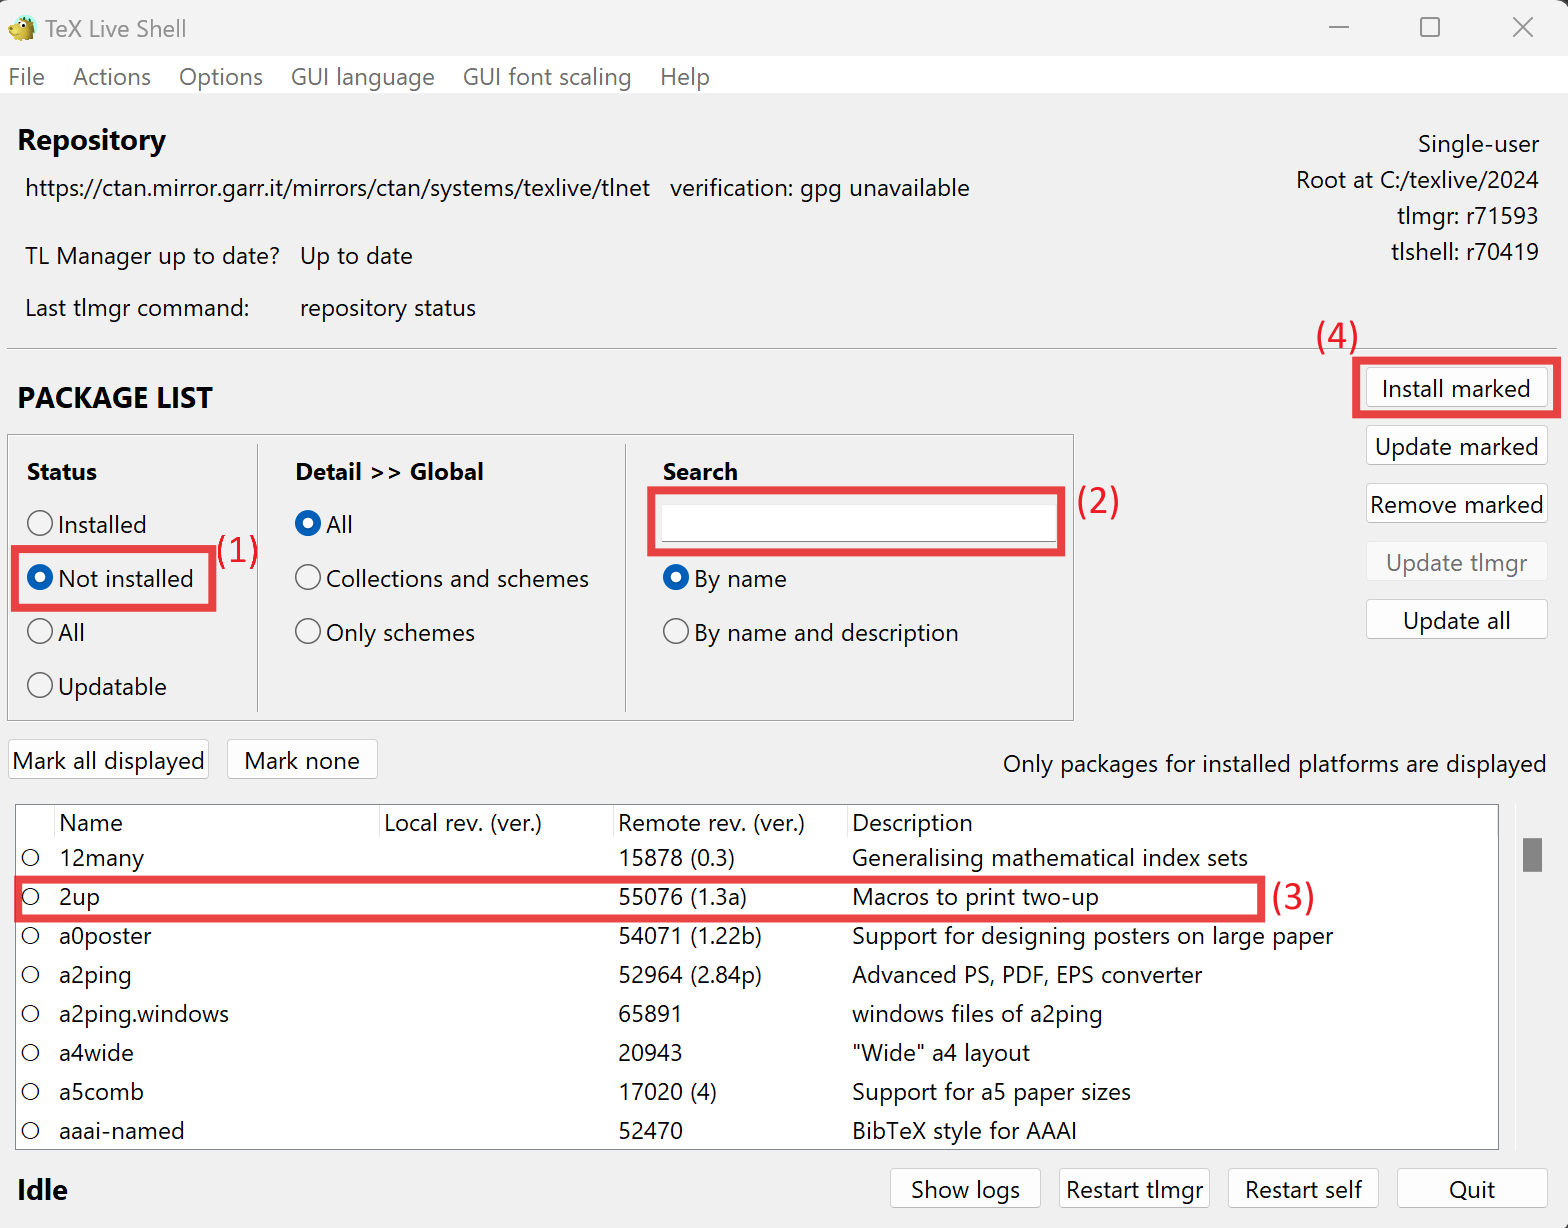
\includegraphics[scale=0.7]{Sezioni/ProcessiDiSupporto/Immagini/installazione_pacchetti.png}
    \caption{Installazione pacchetti LaTeX..}
    \label{fig:installazione_pacchetti}
\end{figure}

\paragraph{Comandi di base}
\label{par:comandi_di_base}
Di seguito vengono elencati i comandi di base che devono essere noti per la stesura di documenti in LaTeX.

\subparagraph{Tabelle}
\begin{lstlisting}

        \begin{table}[!h]
            \begin{tabularx}[| X | c | l | r |]
                \hline

                Intestazione1 &
                Intestazione2 &
                Intestazione3 &
                Intestazione4 \\

                \hline

                prima colonna prima riga   &
                seconda colonna prima riga &
                terza coolonna prima riga  &
                quarta colonna prima riga  &

                \hline

                ...

                \hline
            \end{tabularx}
            \caption{Riassunto contenuto.}
        \end{table}
\end{lstlisting}
Dove:
\begin{itemize}
    \item \lstinline+[!h]+ indica che il posizionamento della tabella nel pdf deve essere dove si trova nel codice.
    
    \item \lstinline+[| X | c | l | r |]+ indica le colonne della tabella.

    \lstinline+|+ indica una riga di separazione tra le colonne.

    \lstinline+X+ indica una colonna che si allarga dinamicamente.

    \lstinline+c+, \lstinline+l+ e \lstinline+r+ indicano rispettivamente colonne in cui il posizionamento del testo è centrale, a sinistra e a destra.

    \item \lstinline+\hline+ crea una linea orizzontale.
\end{itemize}

\subparagraph{Link}
Link a elementi interni alla pagina:
\begin{lstlisting}
    \label[sec:nome]

    ... 

    \hypperref[sec:nome]{nomeLink}
\end{lstlisting}
Dove:
\begin{itemize}
    \item Convezione standard per nominare le label: \texttt{tipoElemento:nome}.
    Dove i possibili tipi di elemento sono: paragraph(par), subparagraph(subpar), section(sec), subsection(subsec) e figure(fig).
\end{itemize}
\noindent Link a elementi esterni alla pagina:
\begin{lstlisting}
    \href{URL}{nomeLink}
\end{lstlisting}

\subparagraph{Listati di codice}
Listati di codice su più righe:
\begin{lstlisting}[mathescape=true]
\begin{lstlisting}
    ...
\$$end{lstlisting}
\end{lstlisting}
\noindent 
Listati di codice inline:
\begin{lstlisting}
    \texttt{code}
    \lstinline+code+
\end{lstlisting}

\subparagraph{Figure}
\begin{lstlisting}
    \begin{figure}[h!]
        \includegraphics[scale=1.2]{pathImmagine}
        \caption{Riassunto immagine.}
        \label{fig:IdFigura}
    \end{figure}
\end{lstlisting}
Dove:
\begin{itemize}
    \item \texttt{[h!]} permette di posizionare la figura nel pdf dove si trova nel codice.
    \item \texttt{scale=x.y} indica la scala da applicare all'immagine.
\end{itemize}

\subparagraph{Inclusione file}
L'inclusione di file .tex permette di dividere un documento in più file rendendone la modifica più semplice.
\begin{lstlisting}
    \input{PercorsoAlFile}
\end{lstlisting} 

\paragraph{Pacchetto LaTeX}
Per rendere i file sorgenti meno complessi è stato deciso di definire un pacchetto LaTeX che contiene:
\begin{enumerate}
    \item La definizione di comandi e ambienti di uso comune.
    \item Le dichiarazioni dei pacchetti usati.
\end{enumerate}
Oltre a diminuire la verbosità dei documenti questo metodo permette di centralizzare la gestione dei pacchetti, dei comandi e degli ambienti semplificando la manutenzione.
I pacchetti usati devono essere installati manualmente usando il processo spiegato nella sezione \hyperref[subpar:TLShell]{TLShell}.
In \hyperref[fig:pacchetto_latex]{Figura \ref{fig:pacchetto_latex}} viene mostrata la struttura del pacchetto LaTeX.
\textbf{Nota bene}: Il pacchetto per poter essere importato deve essere indicato con il comando \lstinline|\usepackage| e il suo percorso deve essere indicato nella variabile di ambiente TEXINPUTS.
La spiegazione della configurazione dell'ambiente per l'utilizzo del pacchetto è spiegata nella sezione \hyperref[par:IDE]{Integrated Development Environment IDE}.
\begin{figure}[!h]
    \dirtree{%
        .1 Packages.
        .2 Immagini.
        .3 logo.jpeg.
        .2 custom.sty.
        .2 TitlePage.tex .
    }
    \caption{Struttura pacchetto LaTeX.}
    \label{fig:pacchetto_latex}
\end{figure}

\subparagraph{Comandi personalizzati}
Nel pacchetto sono definiti i seguenti comandi necessari per la scrittura di un documento:
\begin{enumerate}
    \item \lstinline|\primapagina|\ : inserisce nella posizione di invocazione la pagina iniziale dei documenti.
    Questo comando sfrutta le variabili indicate alla sezione \hyperref[par:struttura_di_base_documenti]{Struttura di base documenti}.
    \item \lstinline|\glossario{<termine>}|\ : modifica lo stile del termine per indicare la sua presenza nel glossario.
    
\end{enumerate}

\subparagraph{Ambienti personalizzati}
Il pacchetto definisce anche i seguenti ambienti necessari per la scrittura di un documento:
\begin{enumerate}
    \item \lstinline|\begin{registromodifiche} ... \end{registromodifiche}|\ :
    permette di definire il registro delle modifiche tralasciando le impostazioni della tabella.
    All'interno di questo ambiente devono essere indicate le righe del \hyperref[par:registro_delle_modifiche]{registro delle modifiche}.
\end{enumerate}

\paragraph{Struttura di base documenti}
\label{par:struttura_di_base_documenti}
Di seguito viene mostrato il codice necessario per la definizione dello scheletro di un documento soggetto al processo di \hyperref[subsec:gestione_della_configurazione]{Gestione della configurazione}:

\begin{lstlisting}
\documentclass[a4paper, 12pt]{article}
\usepackage{custom}

%--------------------VARIABILI--------------------
\def\lastversion{ Versione documento }
\def\title{ Nome documento }
\def\date{ Data }
%------------------------------------------------

\begin{document}

\primapagina

\begin{registromodifiche}

\end{registromodifiche}

\tableofcontents

\newpage
\end{document}
\end{lstlisting}
\textbf{Nota bene}: I valori delle variabili devono seguire le regole indicate nelle sezioni \hyperref[subsec:documentazione]{Documentazione} e \hyperref[par:versione_documenti]{Versione dei documenti}.

\subparagraph{Gestione documenti "lunghi"}
Per rendere più semplice la gestione di documenti molto lunghi il gruppo ha deciso di dividerene il contenuto in più file .tex.
I documenti soggetti a questa divisione sono:
\begin{enumerate}
    \item Norme di progetto.
    \item Analisi dei requisiti.
    \item Piano di progetto.
\end{enumerate}
Ognuno di questi file verrà diviso in sezioni contenute in una cartella avente nome uguale al documento in Pascal case.
Queste cartelle sono contenute nella cartella padre comune \texttt{Sezioni}.
Le sezioni saranno divise a loro volta in sottosezioni contenute nella cartella \texttt{Sottosezioni}.
Inoltre ogni cartella di sottosezione conterrà una cartella chiamata \texttt{Immagini}.
La divisione segue la struttura indicata in \hyperref[fig:struttura_file_lungi]{Figura \ref{fig:struttura_file_lungi}} dove \texttt{F} indica il nome di un file da dividere:

\begin{figure}[!h]
    \dirtree{%
    .1 cartella di F.
    .2 F.tex.
    .2 Sezioni.
    .3 SezioneA.
    .4 SezioneA.tex.
    .4 Sottosezioni.
    .5 Sottosezione\_a.tex.
    .5 Sottosezione\_b.tex.
    .4 Immagini.
    .3 SezioneB.
    .4 SezioneB.tex.
    .4 Sottosezioni.
    .5 Sottosezione\_a.tex.
    .5 Sottosezione\_b.tex.
    .4 Immagini.
    }
    \caption{Struttura file "lunghi".}
    \label{fig:struttura_file_lungi}
\end{figure}


\paragraph{Integrated Development Environment IDE}
\label{par:IDE}
Come IDE per la stesura della documentazione viene utilizzato Visual Studio Code che può essere installato seguendo le istruzioni al seguente link \href{https://code.visualstudio.com/docs/setup/windows}{VsCode}.

Visual Studio Code dispone di un grande numero di estensioni che lo rendono molto versatile.
In particolare sono stati scelti dal gruppo le seguenti estensioni:
\begin{enumerate}
    \item \textbf{LaTeX Workshop}: \href{https://github.com/James-Yu/latex-workshop/wiki}{https://github.com/James-Yu/latex-workshop/wiki}.
    \item \textbf{LTeX+}: \href{ https://ltex-plus.github.io/ltex-plus}{ https://ltex-plus.github.io/ltex-plus}.
\end{enumerate}

\subparagraph{LaTeX Workshop}
Questa estensione permette di integrare la compilazione dei file LaTeX in Visual Studio Code.
LaTeX Workshop richiede che sia installato TeX Live.
Dopo aver installato l'estensione è necessario modificare la procedura di compilazione di modo che vengano cercati i pacchetti usati e i file .tex importati nella cartella Packages.
Per fare ciò è necessario seguire le azioni:
\begin{enumerate}
    \item Aprire Visual Studio Code.
    
    \item Premere la combinazioni di tasti \texttt{Ctrl+,}.
    
    \item Scrivere sulla barra di ricerca il testo \texttt{latex-workshop.tools} \hyperref[fig:texinputs]{Figura \ref{fig:texinputs} (1)}.
    
    \item Cliccare il link \texttt{Edit in settings.json} del primo risultato \hyperref[fig:texinputs]{Figura \ref{fig:texinputs} (2)}.
    
    \item Aggiungere al oggetto tool chiamato \texttt{latexmk} a seguito dell'attributo \texttt{args} l'attributo \texttt{env} indicando il seguente attributo \hyperref[fig:texinputs]{Figura \ref{fig:texinputs} (3)}: 
    \begin{lstlisting}
        "TEXINPUTS":"%WORKSPACE_FOLDER%/Packages;"
    \end{lstlisting}
\end{enumerate}

\begin{figure}[!h]
    \center
    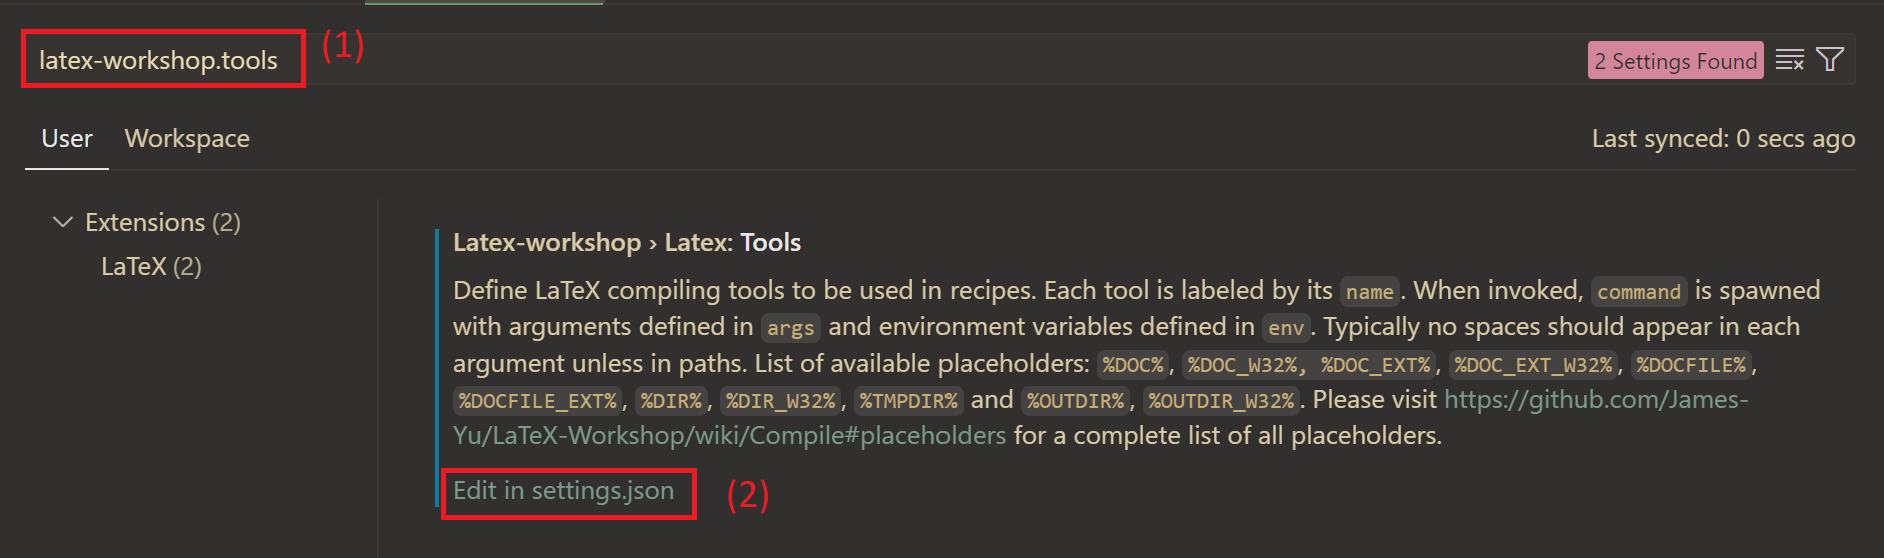
\includegraphics[scale=0.4]{Sezioni/ProcessiDiSupporto/Immagini/texinputs_setup.png}
    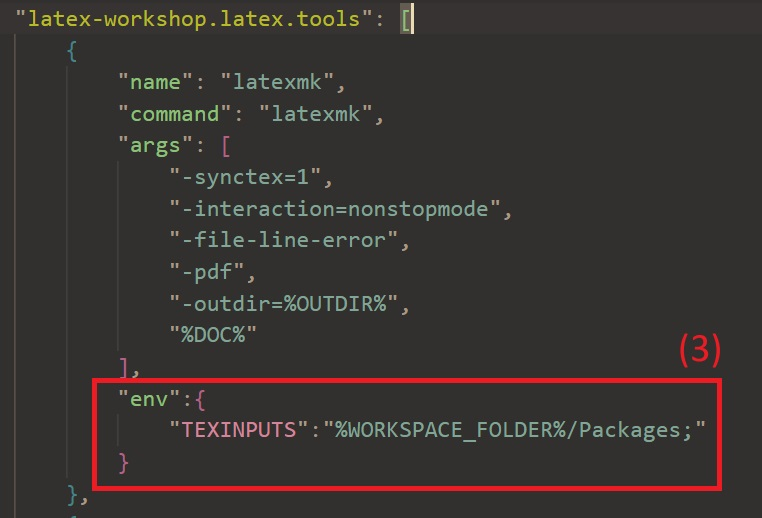
\includegraphics[]{Sezioni/ProcessiDiSupporto/Immagini/texinputs_setup_json.jpg}
    \caption{Modifica impostazioni LaTex Workshop.}
    \label{fig:texinputs}
\end{figure}
\textbf{Nota bene}: Per riuscire ad accedere al pacchetto locale è necessario lavorare in Visual Studio Code usando come "workspace folder" la cartella relativa alla repository.

\subparagraph{LTeX+}
LTeX+ è un'estensione che esegue lo "spell checking" dei documenti .tex per installarla basta cercarla nel marketplace di Visual Studio Code.
Per eventuali problemi di set up le procedure sono spiegate in modo chiaro e dettagliato al link \href{https://ltex-plus.github.io/ltex-plus/vscode-ltex-plus/setting-scopes-files.html}{installazione LTeX+}.

\subsubsection{Gestione della configurazione}
A supporto del processo di gestione della configurazione il gruppo ha scelto l'utilizzo di due strumenti:
\begin{enumerate}
    \item Git: \href{https://git-scm.com/doc}{https://git-scm.com/doc}.
    \item GitHub: \href{https://docs.github.com/en}{https://docs.github.com/en}.
\end{enumerate}

\paragraph{Git}
Git è un Distributed Version Control System DVCS  utilizzabile tramite interfaccia a linea di comando.
I DVCS hanno la caratteristica di permettere ai membri del gruppo di lavoro di mantenere una propria copia locale del repository e della sua storia.
Una volta modificata la copia locale del repository è necessario registrare le modifche nella copia centralizzata del repository.
Le operazioni e gli elementi di base comuni a tutti i DVCS: \textbf{repository}, \textbf{ramo}, \textbf{push}, \textbf{pull}, \textbf{conflitto} e \textbf{commit}.
Nelle sezioni succesive viene mostrato come Git implementa questi concetti e altri concetti caratteristici.

\subparagraph{repository}
Un repository in Git è una cartella contenente:
\begin{enumerate}
    \item Una cartella \texttt{.git} che contiene l'insieme di strutture dati e file necessari per la gestione della storia delle versioni dei file utente.
    \item Un insieme di file utente e cartelle di cui Git deve tenere la storia delle versioni.
\end{enumerate}
In git esistono due diverse declinazioni di repository:
\begin{enumerate}
    \item \textbf{remota}: esiste in un server remoto a cui i membri del team possono attingere tramite le operazioni di push e pull.
    
    \item \textbf{locale}: esiste solo sul file system locale e può essere associata ad un repository remoto usato come default per le operazioni di psuh e pull. 
\end{enumerate} 
Per creare un repository è possibile eseguire uno dei seguenti comandi:
\begin{lstlisting}
    git clone <URL>
    git init <NomeRepository>
\end{lstlisting}
Dove:
\begin{enumerate}
    \item Il primo comando permette di copiare la repository remota nella current working directory proprio file system.
    \item Il secondo comando permette di creare una repository nella current working directory nel proprio file system.
\end{enumerate}

\subparagraph{commit}
\label{subpar:commit}
Un commit rappresenta una istantanea del contenuto di uno o più file utente di cui è stata indicata l'esistenza a Git.
In Git ogni commit è associato alle seguenti informazioni:
\begin{enumerate}
    \item \textbf{hash SHA-1}: sequenza di 40 caretteri alfanumerici che identifica univocamente il commit all'interno del repository.
    \item \textbf{autore}.
    \item \textbf{data di creazione}.
    \item \textbf{messaggio}: usato per segnalare cosa fa il contenuto del commit.
    \item \textbf{commit padre}: hash SHA-1 dei commit padre.
\end{enumerate}
I commit sono quindi messi in relazione "padre-figlio" da Git andando a creare un albero.
L'unico commit che non ha padre è il primo commit chiamato \textbf{commit radice}.
I commit con più di un padre sono dei commit generati da operazioni di \hyperref[subpar:merge]{merge}.
Il comando Git per generare un commit con commento è:
\begin{lstlisting}
    git commit -m "<commento>"
\end{lstlisting}
Per comprendere meglio i commit leggere sezione \hyperref[subpar:3_aree_git]{3 aree di Git}.
Questo comando utilizza come commit padre il commit foglia del ramo corrente. 

\subparagraph{ramo}
\label{subpar:branch}
Un ramo in Git è un commit a cui è stata associata un etichetta mobile che funziona da alias per lo stesso.
Tramite questa etichetta mobile è possibile fare riferimento al commit ad essa associato.
Un ramo è un etichetta mobile nel senso che Git la sposta in automatico quando viene generato un commit figlio.
Questo crea una biforcazione nella storia dei commit(ramo) dove l'etichetta punta sempre all'ultimo commit(foglia) del nuovo flusso.

Git mantiene internamente un puntatore all'etichetta del ramo corrente chiamato commit \textbf{HEAD}.
Così facendo riesce ad operare nel modo atteso quando si eseguono comandi che agiscono rispetto al ramo corrente.
Git permette di ottenere riferimenti a commit padre del commit HEAD tramite le seguenti sintassi:
\begin{lstlisting}
    # riferimento al commit padre di HEAD
    # si possono concatenare arbitrari ^
    HEAD^

    # riferimento ad n-esimo parente di HEAD
    HEAD~n
\end{lstlisting}
 

Per creare un ramo esiste il comando:
\begin{lstlisting}
    git branch <nomeRamo>
\end{lstlisting}
Per eliminare un ramo esiste il comando:
\begin{lstlisting}
    # il ramo non deve avere commit
    git branch -d <nomeRamo>

    # il ramo puo avere commit
    git branch -D <nomeRamo>
\end{lstlisting}
Per spostarsi in un ramo esiste il comando:
\begin{lstlisting}
    git checkout <nomeRamo>
\end{lstlisting}
Per ottenere una lista dei rami del repository locale esiste il comando:
\begin{lstlisting}
    git branch
\end{lstlisting}
Per ottenere una lista dei rami dei repository locale e remoto è necessario applicare l'opzione \texttt{-a} al comando precedente.


\subparagraph{3 aree di Git}
\label{subpar:3_aree_git}
Git lavora su tre diversi livelli:
\begin{enumerate}
    \item \textbf{Commit HEAD}: rappresenta il ramo corrente.
    Per gestire il ramo corrente esistono i seguenti comandi:
    \begin{lstlisting}
    # modifica etichetta ramo correte usando il
    # commit indicato le modifiche vengono 
    # eliminate dal file system
    git reset --hard <hashCommit>

    # modifica etichetta ramo correte usando il
    # commit indicato le modifiche tornano 
    # nell'area di staging 
    git reset --soft <hashCommit>

    # ottenere la storia dei commit 
    # del ramo corrente
    git log --graph
    
    # ottenere la storia dei commit 
    # di tutti i rami
    git log --all --graph

    # ottenere differenze con area di staging
    git diff --cached
    
    # ottenere differenze con albero di lavoro
    git diff HEAD
    \end{lstlisting}
    
    \item \textbf{Area di staging}: anche chiamata indice o cache, è una struttura dati dinamica che contiene le modifiche ai file utente che Git deve aggiungere nel prossimo commit.
    
    Di seguito vengono mostrati i comandi per la gestione dell'area di staging:
    \begin{lstlisting}
    # aggiunge file
    git add <percorsoFile>

    # rimuove i file separati da ,
    git checkout -- <files>

    # ottenere differenze con albero di lavoro
    git diff 
    \end{lstlisting}
    
    \item \textbf{Albero di lavoro}: albero di cartelle e file che Git "conosce" e quindi ritiene come facenti parte del repository.
    
    Questi file e cartelle vengono chiamati \textbf{file tracciati} e devono per forza essere memorizzati all'interno della cartella relativa al repository.

    Un file diventa tracciato quando è passato dall'area di staging.
\end{enumerate}


\subparagraph{push}
\label{subpar:push}
L'operazione di push permette di pubblicare le modifiche apportate ad un repository locale al repository remoto a cui è associato.
Le declinazioni del comando di Git che permette di eseguire un push sono:
\begin{lstlisting}
    # pubblica il contenuto del ramo locale 
    # corrente nel ramo remoto indicato
    git push origin <ramoDestinazione> 

    # pubblica il contenuto del ramo locale
    # indicato nel ramo remoto indicato
    git push <ramoSorgente> origin <ramoDestinazione>
\end{lstlisting}   
Dove \texttt{origin} è il nome di default del riferimento al repository remoto e può essere gestiti usando i comandi:
\begin{lstlisting}
    # aggiunge nuovo riferimento remoto
    git remote add <nome> <URL>

    # rimuove il riferimento remoto
    git remote remove <nome>

    # modifica il riferimento remoto
    git remote set-url <nome> <URL>
\end{lstlisting}

\subparagraph{pull}
\label{subpar:pull}
L'operazione di pull permette aggiornare un repository locale con le modifiche registrate al repository remoto a cui è associato.
Git per eseguire un operazione di pull mette a dispozione il seguente comando:
\begin{lstlisting}
    # esegue il pull del ramo remoto indicato
    # nel ramo locale corrente
    git pull origin <nomeRamo>
\end{lstlisting}
In realà il comando \lstinline|git pull| è un comando composto che accorpa i comandi:
\begin{enumerate}
    \item \lstinline|git fetch origin <nomeRamo>|: recupera localmente il ramo remoto indicato.
    \item \lstinline|git merge <nomeRamo>|.
\end{enumerate}

\subparagraph{merge}
\label{subpar:merge}
L'operazione di merge esegue una fusione di due o più rami sorgente verso un ramo di destinazione.
A seguito dell'operazione di merge la cronologia del ramo di destinazione conterrà le modifiche dei rami sorgente.
In una fusione possono accadere le seguenti situazioni:
\begin{enumerate}
    \item I commit HEAD dei rami contengono file con nomi uguali ma contenuto diverso.
    In questo caso sorge un \textbf{conflitto}.

    \item Non esistono conflitti.

    \item Il commit HEAD del ramo di destinazione è in dietro rispetto ai commit HEAD dei rami sorgente.
    In questo caso avviene un \textbf{fast-forward} e Git risolve il merge in automatico spostando l'etichetta del ramo di destinazione.
\end{enumerate}
Nei primi due casi Git ci guiderà nell'assemblaggio di un nuovo commit HEAD per il ramo di destinazione chiamato \textbf{merge commit}.

Per eseguire un merge è necessario usare il comando:
\begin{lstlisting}
    # merge ramo indicato nel ramo corrente
    git merge <nomeAlbero>
\end{lstlisting}

Nel caso in cui esista un conflitto Git richiede la risoluzione manuale dello stesso tramite la modifica dei file.
Git indica questa situazione nella console in cui appare la keyword \texttt{MERGING} che indica il fatto che siamo nel mezzo di un operazione di fusione.
In questa situazione il comando \lstinline|git diff| ci mostra i conflitti.
Per uscire dallo stato di \texttt{MERGING} eliminando l'operazione di merge è possibile eseguire il comando \lstinline|git merge --abort|.

Una volta sistemato il conflitto si rientra nel caso in cui non esistano conflitti.
In questo caso è necessario eseguire il \textbf{merge commit} che avrà come commit padre i  commit HEAD del ramo di destinazione e del 
ramo sorgente.

\paragraph{GitHub}
GitHub permette la memorizzazione e la gestione di repository Git.
Attorno alle funzionalità offerte da Git implementa nuove funzionalità e servizi a supporto dello sviluppo di progetti.

\subparagraph{GitHub organization}
GitHub offre degli account particolari chiamati \textbf{organization account} che permettono definire più repository pubblici a cui uno stesso gruppo di lavoro ha accesso.
Il gruppo ha deciso di utilizzare un account di questo tipo dato che è pensato per la realizzazione di progetti.
L'account del gruppo si trova al link \href{https://github.com/ALT-F4-eng/}{https://github.com/ALT-F4-eng/}.

Nell'account sono state definite le seguenti repository pubbliche:
\begin{enumerate}
    \item \href{https://github.com/ALT-F4-eng/SorgentiDocumentazione}{SorgentiDocumentazione}: contiene la documentazione scritta in LaTeX.
    \item \href{https://github.com/ALT-F4-eng/Documentazione}{Documentazione}: contiene i documenti pdf e il sito web per la loro pubblicazione.
\end{enumerate}

\subparagraph{Gestione dei rami}
GitHub permette di gestire tramite la pagina web del repository i rami in esso definiti.
In particolare permette l'esecuzione delle seguenti operazioni:
\begin{enumerate}
    \item \textbf{Creazione ramo}
    
    La creazione di un ramo segue le operazioni:
    \begin{enumerate}
        \item Selezionare la scheda "Code".
        \item Premere il bottone "Branches".
        \item Premere il bottone "New branch".
        \item Indicare il nome del nuovo ramo.
        \item Indicare il ramo di partenza tramite il menù a tendina con label "Source".
        \item Premere il bottone "Create new branch".
    \end{enumerate}

    \item \textbf{Eliminazione ramo}
    
    L'eliminazione di un ramo segue le operazioni:
    \begin{enumerate}
        \item Selezionare la scheda "Code".
        \item Premere il bottone "Branches".
        \item Trovare il ramo da eliminare.
        \item Premere il bottone raffigurante un cestino.
    \end{enumerate}

\end{enumerate}

\subparagraph{Issue}
\label{subpar:ITS}
GitHub fornisce un ITS ovvero un sistema che permette di registrare e gestire le richieste di modifica.
Le richieste di modifica sono rappresentate tramite il concetto di \textbf{issue}.
Un issue è composta dai seguenti elementi:
\begin{enumerate}
    \item \textbf{Titolo}: nome della richiesta di modifica.
    
    \item \textbf{Id}: numero univoco che identifica la richiesta di modifica all'interno del sistema.
    
    \item \textbf{Stato}: indica lo stato attuale della richiesta di modifica tra gli stati che essa può attraversare durante il suo ciclo di vita.
    
    \item \textbf{Etichetta}: rappresenta in modo schematico la tipologia di richiesta di modifica.
    
    \item \textbf{Assegnatario}: indica il membro del gruppo di lavoro che sta implementando la richiesta di modifica.
    
    \item \textbf{Milestone}: indica la \glossario{milestone} a cui la richiesta di modifica appartiene.
    
    \item \textbf{Commenti}: lista di commenti che specificano con più precisione la richiesta di modifica. 
\end{enumerate}
Di seguito vengono indicate l'insieme di operazioni che possono essere eseguite su un issue:
\begin{enumerate}
    \item \textbf{Creazione}
    \label{item:creazione_issue}
    
    Per creare una issue è necessario eseguire i seguenti passi a partire dalla pagina web del repository:
    \begin{enumerate}
        \item Selezione finestra "Issues".
        \item Cliccare tasto "New issue".
        \item Inserire titolo della issue.
        \item Inserire descrizione della issue.
        La descrizione supporta un linguaggio di markup chiamato Markdown, questo aiuta a rendere la descrizione più strutturata.

        La descrizione di una issue deve seguire la struttura:
        \begin{lstlisting}
        # File da modificare
        <percorso primo file>
        <percorso secondo file>
        ...

        # Cosa fare
        - [ ] <primo compito>
        - [ ] <secondo compito>
        ...

        # Ruolo
        <ruolo>

        # Ore preventivate
        <ore preventivate>
        \end{lstlisting}
        Il significato del codice viene indicato nella sezione \hyperref[subpar:markdown]{Markdown}.

        \item Assegnare una o più etichette.
        \item Assegnare il progetto chiamato \textbf{ArtificalQI}.
        \item Cliccare il pulsante "Submit new issue".
    \end{enumerate}
    
    \item \textbf{Eliminazione}
    
    Per eliminare una issue è necessario eseguire i seguenti passi a partire dalla pagina web del repository:
    \begin{enumerate}
        \item Selezionare finestra "Issues".
        \item Selezionare la issue che si vuole eliminare.
        \item Cliccare il bottone "Delete issue".
    \end{enumerate}

    \item \textbf{Chiusura}
    
    Per chiudere una issue è necessario eseguire i seguenti passi a partire dalla pagina web del repository:
    \begin{enumerate}
        \item Selezionare finestra "Issues".
        \item Selezionare la issue che si vuole chiudere.
        \item Cliccare il bottone "Close issue".
    \end{enumerate}
    Chiudere una issue equivale a indicare che la richiesta di modifica che rappresenta è stata implementata e verificata correttamente.

    \item \textbf{Modifica}
    
    Per modificare una issue è necessario eseguire i seguenti passi a partire dalla pagina web del repository:
    \begin{enumerate}
        \item Selezionare finestra "Issues".
        \item Selezionare la issue che si vuole modificare.
        \item Ora è possibile modificare: commenti, titolo, etichetta, assegnatario, progetto ecc.
    \end{enumerate}

    \item \textbf{Commentare un issue}
    
    Per aggiungere un commento ad una issue è necessario eseguire i seguenti passi a partire dalla pagina web del repository:
    \begin{enumerate}
        \item Selezionare finestra "Issues".
        \item Selezionare la issue che si vuole commentare.
        \item Scrivere il commento nella barra con label "Add a comment"(I commenti supportano il linguaggio Markdown).
        \item Premere il bottone "Comment"
    \end{enumerate}
\end{enumerate}

\subparagraph{Markdow}
\label{subpar:markdown}
Markdown è un linguaggio di markup che permette di strutturare il testo.
Gli elementi di base utili per l'utilizzo di questo linguaggio sono:
\begin{itemize}
    \item \textbf{Check list}
    \begin{lstlisting}
    - [ ] elemento 1
    - [ ] elemento 2
    - [ ] elemento 3
    ...
    \end{lstlisting}

    \item \textbf{Lista non numerata}
    \begin{lstlisting}
    - elemento 1
    - elemento 2
    - elemento 3
    ...
    \end{lstlisting}

    \item \textbf{Lista numerata}
    \begin{lstlisting}
    1. elemento 1
    2. elemento 2
    3. elemento 3
    ...
    \end{lstlisting}

    \item \textbf{Headings}
    \begin{lstlisting}
    # Titolo livello 1
    ## Titolo livello 2
    ### Titolo livello 3
    ...
    \end{lstlisting}
    
\end{itemize}

\subparagraph{Etichette}
Di seguito viene fornita una lista delle etichette relative al repository SorgentiDocumentazione:
\begin{enumerate}
    \item \textbf{bug}: riguarda la sistemazione di un documento.
    \item \textbf{enhancement}: riguarda l'implementazioni di automazioni della gestione e organizzazione di progetto.
    \item \textbf{requirement}: riguardano il documento di analisi dei requisiti.
    \item \textbf{documentation}: riguardano gli altri documenti.
\end{enumerate}

\subparagraph{pull request}
Una pull request in GitHub è una richiesta di merge di un ramo sorgente verso un ramo destinazione.
Di seguito vengono elencate e descritte le operazioni per la gestione delle pull requet:
\begin{enumerate}
    \item \textbf{Creazione}\label{item:creazione_pull_request}
    
    Per creare una pull request bisogna seguire questi passaggi a partire dal sito web del repository:
    \begin{enumerate}
        \item Selezionare la scheda "Pull requests".
        \item Premere il pulsante "New pull request".
        \item Selezionare il ramo di destinazione tramite il menù a tendina "base:".    
        \item Selezionare il ramo di sorgente tramite il menù a tendina "compare:".
        \item Premere il pulsante "Create pull request".
    \end{enumerate}
    
    \item \textbf{Chiusura}\label{item:chiusura_pull_request}
    
    Per chiudere una pull request bisogna seguire questi passaggi a partire dal sito web del repository:
    \begin{enumerate}
        \item Selezionare la scheda "Pull requests".
        \item Selezionare la pull request che si vuole chiudere.
        \item Cliccare il bottone "Close pull request".
    \end{enumerate}

    \item \textbf{Approvazione} \label{item:approvazione_pull_request}
    
    L'approvazione di una pull request implica l'esecuzione dell'operazione di merge dal ramo sorgente al ramo destinazione.
    Come nel caso dell'esecuzione di un merge nel repository locale possono presentarsi tre casi:

    \begin{enumerate}
        \item \textbf{Esistono dei conflitti}.
        \item \textbf{Fast-forward}.
        \item \textbf{Non esistono dei conflitti}.
    \end{enumerate}

    Nel primo caso sarà necessario risolvere i conflitti eseguendo le seguenti operazioni a partire dalla pagina relativa alla pull request:
    \begin{enumerate}
        \item Cliccare il bottone "Resolve conflicts".
        \item GitHub mostrerà una lista composta dai documenti che sono in conflitto.
        
        Per ognuno dei conflitti viene indicata la differenza tra il documento presente nel ramo sorgente e quello presente nel ramo destinazione.

        \item Una volta sistemato il conflitto premere il bottone "Mark as resolved".
        
        \item Ripetere il passo 3. finchè tutti i conflitti sono risolti.
        
        \item Cliccare il bottone "Commit merge".
        
        \item Ora la procedura si ricollega ai casi \textbf{Fast-foward} e \textbf{Non esistono confilitti}.
    \end{enumerate}    

    Nel caso di \textbf{Fast-forward} o nel caso in cui \textbf{Non esistono dei conflitti} seguire i passi:
    \begin{enumerate}
        \item Cliccare il bottone "Merge pull request".
        \item Indicare un commento per il merge commit.
        \item Cliccare il pulsante "Confirm merge".
        \item Cliccare il pulsante "delete branch".
    \end{enumerate}
\end{enumerate}


\subparagraph{Project}
\label{subpar:project}
GitHub permette di raggruppare le issue in progetti.
Un progetto può offrire più "rappresentazioni" dell'insieme di issue che contiene.
Le rappresentazioni si basano sul valore di proprietà associate alle issue(assegnatario, etichetta, milestone ecc).
I progetti introducono anche la possibilità di creare proprietà personalizzate.
In particolare esistono 3 tipologie di rappresentazioni:
\begin{enumerate}
    \item \textbf{Task-board}
    
    Una task-board è una tabella composta da un insieme di colonne.
    Ogni colonna corrisponde a un valore per una proprietà e contiene tutte le issue che hanno tale valore per la proprietà stessa.
    Ogni membro del team può modificare il valore della proprietà per una issue spostandola nella rispettiva colonna.

    Per una guida più completa su questa tipologia di rappresentazione viene lasciato il seguente \href{https://docs.github.com/en/issues/planning-and-tracking-with-projects/customizing-views-in-your-project/customizing-the-board-layout}{link}.

    \item \textbf{Table layout}
    
    Le issue vengono organizzate in una tabella.
    Ogni riga contiene una issue.
    Le colonne contengono i valori delle proprietà selezionate delle issue. 
    Questa rappresentazione permette di eseguire diverse operazioni sulle issue quali: ordinamento per proprietà, raggruppamento per proprietà, separazione per proprietà ecc.
    
    Per una guida più precisa alle operazioni esistenti e come applicarle viene lasciato il seguente \href{https://docs.github.com/en/issues/planning-and-tracking-with-projects/customizing-views-in-your-project/customizing-the-table-layout}{link}.

    \item \textbf{Road map}
    
    Le issue vengono organizzate in un \glossario{diagramma di Gantt}.
\end{enumerate}
Il gruppo ha deciso di utilizzare tre rappresentazioni del progetto:
\begin{enumerate}
    \item \textbf{Progetto}
    
    task-board definita sulla proprietà \hyperref[subpar:github_stato]{Stato} che viene utilizzata come project backlog.

    \item \textbf{Sprint backlog} \label{item:sprint_backlog}
    
    task-board generata applicando un filtro sul valore della proprietà \textbf{Iteration} delle issue.
    Questo filtro seleziona solo le issue che hanno per valore lo sprint attuale per la proprietà \textbf{Iteration}.
    Questa task-board contiene quindi le richieste di modifica da portare a termine nello sprint corrente.
    Per informazioni sulle proprietà personalizzate leggere la sezione \hyperref[subpar:proprietà_personalizzate]{Proprietà personalizzate}.

    \item \textbf{Tabella progetto}
    
    Un table layout che rappresenta il project backlog in modo alternativo per semplificare l'assegnazione di valori alle proprietà delle issue.
\end{enumerate}

\subparagraph{Proprietà personalizzate}
\label{subpar:proprietà_personalizzate}
Le proprietà personalizzate anche chiamate issue possono essere gestiste a partire dalla pagina di progetto.
Per accedere alle proprietà personalizzate è necessario eseguire i seguenti passi:
\begin{enumerate}
    \item Spostarsi sulla pagina di progetto.
    \item Premere il pulsante "...".
    \item Selezionare l'opzione "Settings".
    \item Ora è possibile:
    \begin{itemize}
        \item \textbf{Aggiungere un campo}.
        \begin{enumerate}
            \item Selezionare il pulsante "+ New field".
            \item Indicare il nome del campo.
            \item Indicare il tipo del campo.
            \item Cliccare il pulsante "Save".
        \end{enumerate}

        \item \textbf{Modificare un campo}.
        \begin{enumerate}
            \item  Selezionare il campo da modificare.
            \item Aggiungere un possibile valore o eliminarne uno esistente.
        \end{enumerate}
    \end{itemize}
\end{enumerate}
Per assegnare un valore a una proprietà personalizzata di una issue è necessario eseguire i seguenti passaggi:
\begin{enumerate}
    \item Spostarsi sulla pagina di progetto.
    \item Selezionare la vista del progetto chiamata "TabellaProgetto".
    \item Individuare la issue per cui si vuole assegnare un valore.
    \item Spostasi sulla colonna nominata come il campo personalizzato.
    \item Cliccare il pulsante "$\triangledown$".
    \item Selezionare il valore per la proprietà tra le scelte del menù a tendina.
\end{enumerate}
Le proprietà utilizzate dal gruppo sono:
\begin{enumerate}
    \item Sprint: usata per associare le issue agli sprint.
    \item Priority: usata per indicare la priorità delle issue.
\end{enumerate}

\subparagraph{Stato}
\label{subpar:github_stato}
Lo stato di una issue è una proprietà personalizzata che corrisponde allo stato della richiesta di modifica che la issue rappresenta.
I valori che questa proprietà può assumere sono:
\begin{enumerate}
    \item \textbf{To do}.
    \item \textbf{In progress}.
    \item \textbf{To review}.
    \item \textbf{In review}.
    \item \textbf{Re open}.
    \item \textbf{Done}.
\end{enumerate}
Per informazioni dettagliate sullo stato delle richieste di modifica leggere la sezione \hyperref[par:ciclo_vita_richieste_di_modifica]{Ciclo di vita delle richieste di modifica}.

\subparagraph{Presa in carico di una modifica}
\label{subpar:presa_carico_modifica}
Per poter prendere in carico una modifica essa deve appartenere alla rappresentazione \hyperref[item:sprint_backlog]{Sprint backlog}.

Per prendere in carico l'esecuzione di una modifica è necessario trascinarla dalla colonna di appartenenza alla colonna che indica l'esecuzione della stessa.

In accordo con la sezione \hyperref[par:ciclo_vita_richieste_di_modifica]{Ciclo di vita delle richieste di modifica} le possibili colonne di partenza sono: "To do" e "Re open" mentre l'unica colonna di destinazione possibile è "In progress".

\subparagraph{Presa in carico di una verifica}
\label{subpar:presa_carico_verifica}
Per poter prendere in carico una verifica essa deve appartenere alla rappresentazione \hyperref[item:sprint_backlog]{Sprint backlog}.

Per prendere in carico una verifica il Verificatore deve trascinarla dalla colonna "To review" alla colonna "In review".

\subparagraph{Richiesta di verifica}
\label{subpar:github_richiesta_di_verifica}
Per richiedere la verifica di una modifica è necessario \hyperref[item:creazione_pull_request]{aprire una pull request} avente come:
\begin{itemize}
    \item \textbf{Ramo sorgente}: il ramo contenete la modifica da verificare che deve seguire le indicazioni fornite nella sezione \hyperref[subpar:strategia_di_branching_documenti]{Strategia di branching}.
    
    \item \textbf{Ramo destinazione}: il ramo \texttt{develop}.
\end{itemize}

\subparagraph{Accettazione modifiche}
\label{subpar:accettazione_modifiche}
Per accettare le modifiche di cui è stata richiesta la verifica è necessario eseguire il \hyperref[item:approvazione_pull_request]{merge della pull request}.
Ed eliminare il ramo sorgente della pull request.

Per informazioni sulla risoluzione dei conflitti nella strategia di branching scelta dal gruppo leggere la sezione \hyperref[subpar:risoluzione_dei_conflitti]{Risoluzione dei conflitti}.


\subparagraph{Rifiuto modifiche}
\label{subpar:rifiuto_modifiche}
Per rifiutare le modifiche di cui è stata richiesta la verifica è necessario \hyperref[item:chiusura_pull_request]{chiudere la pull request}.

Il verificatore in questo caso ha l'onere di indicare in un \hyperref[item:commentare_issue]{commento della issue} i miglioramenti da apportare la modifica affinchè venga accettata nella verifica successiva.

\subparagraph{Pubblicazione dei documenti}
La pubblicazione dei documenti avviene al raggiungimento di ogni baseline.
Questa operazione è automatizzata tramite il meccanismo delle \hyperref[subsebsec:github_action]{GitHub action}.
In particolare i documenti vengono pubblicati seguendo la stessa struttura del repository contenente i sorgenti.

\subparagraph{Distribuzione dei documenti}
La distribuzione dei documenti avviene tramite un sito web reso accessibile tramite il servizio di hosting offerto da GitHub.
Il sito segue la struttura indicata in \hyperref[fig:sito_docs]{Figura \ref{fig:sito_docs}}.

\begin{figure}[!h]
\dirtree{%
    .1 repository Documenti.
    .2 Js.
    .3 repoTree.js.
    .3 script.js.
    .2 Assets.
    .2 Style.
    .3 style.css.
    .2 index.html.
}
\caption{Struttura sito web.}
\label{fig:sito_docs}
\end{figure}

\subsubsection{Github action}
Le GitHub action sono un meccanismo messo a disposizione da GitHub che permette di automatizzare dei compiti dei diversi processi di sviluppo.
L'automazione avviene indicando un flusso di lavoro che viene eseguito da GitHub alla necessità su un container.

\paragraph{Teoria}

\subparagraph{Workflow}
Ogni workflow ha un proprio nome che viene usato da GitHub per identificarlo nei report delle esecuzioni.
Una workflow è composto dai seguenti elementi fondanti:
\begin{itemize}
    \item \textbf{events}: ogni workflow risponde a determinati eventi sul repository a cui esso appartiene.
    Di seguito viene indicato un link alla lista completa dei possibili eventi: \href{https://docs.github.com/en/actions/writing-workflows/choosing-when-your-workflow-runs/events-that-trigger-workflows}{events}.

    \item \textbf{jobs}: insieme di compiti che devono essere eseguiti in risposta all'evento.
    Di default i job vengono eseguiti in parallelo su container diversi.
\end{itemize}

\subparagraph{Jobs}
Ogni job ha un nome che viene usato da GitHub per identificarlo nei report delle esecuzioni.
Un job è composto dai seguenti elementi fondanti:

\begin{itemize}
    \item \textbf{env}: una o più variabili d'ambiente accessibili all'interno del job stesso.
    runner: l'identificativo del runner(container) hostato da GitHub che deve eseguire il job.
    GitHub offre diversi container che variano nella versione/tipo di OS utilizzato.
    Di seguito viene indicato un link che contiene la lista dei runner hostati da GitHub \href{https://docs.github.com/en/actions/writing-workflows/workflow-syntax-for-github-actions#choosing-github-hosted-runners}{runners}. 
    \item \textbf{steps}: insieme di compiti atomici che formano il job e vengono eseguiti  sequenzialmente sul runner.
\end{itemize}

\subparagraph{Step}
Ogni step è identificato da GitHub tramite un nome.
Uno step è composto dai seguenti componenti presenti in modo mutuamente esclusivo:
\begin{itemize}
    \item \textbf{action}: nome di una GitHub action appartenente al marketplace.
    Il marketplace delle GitHub action si trova al link \href{https://github.com/marketplace?type=actions}{actions}.
    
    \item \textbf{comandi}: uno o più comandi che vengono eseguiti nel runner.
\end{itemize}

\paragraph{Pratica}

\subparagraph{Definizione workflow}
I workflow devono essere definiti nella cartella .github/workflows del repository.
Ogni workflow viene specificato in un apposito file che contiene la definizione del workflow tramite il linguaggio YAML.
I file dei workflow hanno quindi estensione .yaml.
La sintassi per la definizione di un workflow è:
\begin{lstlisting}
name: <nomeWorkflow>

on:
    <evento>
jobs:
    <jobs>
\end{lstlisting}

\subparagraph{Definizione job}
Un job viene definito seguendo la sintassi:
\begin{lstlisting}
<nome>:
    if: <condizione>
    runs-on: <runner>
    env:
        <env1>
        <env2>
        ...
    steps:
        <step1>
        <step2>
        ...
\end{lstlisting}
Dove:
\begin{itemize}
    \item La condizione determina se il job viene eseguito o meno e serve per analizzare aspetti più specifici dell'evento(non è obbligatoria).
    
    \item Le variabili d'ambiente(env) vengono definite usando la sintassi:
    \begin{lstlisting}
    <nome>: <valore>
    \end{lstlisting}
\end{itemize}

\subparagraph{Definizione step}
Uno step che utilizza una action viene definito seguendo la sintassi:
\begin{lstlisting}
    name: <nomeStep>
    uses: <nomeAction>
        with:
            <arg1>
            <arg2>
            ...
\end{lstlisting}
Dove:
\begin{itemize}
    \item Il nome dell'action segue solitamente la seguente forma standard: 
    \begin{lstlisting}
    <proprietarioRepository>/<nomeRepository>@<vers>
    \end{lstlisting}
    Dove la repository è quella in cui è definita la action da utilizzare e la versione è appunto la versione della action che si vuole usare.
    \item  Ogni argomento viene indicato seguendo la sintassi: \texttt{<nome>: <valore>}.
\end{itemize}
Le action sono solitamente documentate in modo estensivo nel file README.md del repository che le contiene.
In caso in cui ciò non sia vero all'interno del repository deve esistere un file chiamato action.yaml(ogni action deve averlo così GitHub la riconosce come tale) che definisce: argomenti e output della action.

\paragraph{Variabili GitHub}
Le variabili definite a livello di repository sono accessibili da parte di tutte le GitHub action contenute nel repository stesso.
Le variabili permettono di modificare i valori usati dalle action senza dover modificare il file in cui esse sono definite.

\subparagraph{Definizione}
Per definire una variabile a livello di repository è necessario seguire i passaggi:
\begin{enumerate}
    \item Spostarsi sulla pagina della repository in cui si vuole definire la variabile.
    \item Selezionare la scheda "Settings".
    \item Selezionare la voce "Secrets and variables" nel menù laterale.
    \item Selezionare la sottovoce "Actions" del menù a tendina.
    \item Selezionare la scheda "Variables".
    \item Cliccare il bottone "New repository variable" 
    \item Indicare Nome e Valore della variabile.
    \item Cliccare il pulsante "Add variable".
\end{enumerate}

\subparagraph{Gestione}
Per modificare una variabile definita a livello di repository è necessario seguire i passaggi:
\begin{enumerate}
    \item Spostarsi sulla pagina della repository in cui si vuole modificare una variabile.
    \item Selezionare la scheda "Settings".
    \item Selezionare la voce "Secrets and variables" nel menù laterale.
    \item Selezionare la sottovoce "Actions" del menù a tendina.
    \item Selezionare la scheda "Variables".
    \item Cliccare il bottone con l'icona della matita che compare a fianco alla variabile.
    \item Indicare Nome e/o Valore della variabile.
    \item Cliccare il pulsante "Update variable".
\end{enumerate}

\paragraph{Secrets GitHub}
I secrets sono delle variabili "speciali" il cui valore viene crittografato e mantenuto da GitHub.
Il valore di un secret definito a livello di repository è accessibile alle GitHub action che vi appartengono.
Una volta assegnato un valore ad un secret esso non è più visibile dalle impostazioni del repository, tuttavia il suo valore può essere modificato.

\subparagraph{Definizione}
Per definire un secret a livello di repository è necessario seguire i passaggi:
\begin{enumerate}
    \item Spostarsi sulla pagina della repository in cui si vuole definire il secret.
    \item Selezionare la scheda "Settings".
    \item Selezionare la voce "Secrets and variables" nel menù laterale.
    \item Selezionare la sottovoce "Actions" del menù a tendina.
    \item Selezionare la scheda "Secrets".
    \item Cliccare il bottone "New repository secret" 
    \item Indicare Nome e Valore del secret.
    \item Cliccare il pulsante "Add secret".
\end{enumerate}

\subparagraph{Gestione}
Per modificare un secret definito a livello di repository è necessario seguire i passaggi:
\begin{enumerate}
    \item Spostarsi sulla pagina della repository in cui si vuole modificare un secret.
    \item Selezionare la scheda "Settings".
    \item Selezionare la voce "Secrets and variables" nel menù laterale.
    \item Selezionare la sottovoce "Actions" del menù a tendina.
    \item Selezionare la scheda "Secrets".
    \item Cliccare il bottone "Manage organization secrets".
    \item Cliccare il bottone con l'icona della matita che compare a fianco del secret.
    \item Indicare il nuovo Nome e/o Valore del secret.
    \item Cliccare il pulsante "Save changes".
\end{enumerate}

\paragraph{Pubblicazione dei documenti}
\label{par:pubblicazione_documenti}
La pubblicazione utilizza un workflow definito nel file \texttt{PublicazioneDocumenti.yaml}.
Questo workflow viene eseguito ogni volta che avviene la pubblicazione di un commit nel ramo \texttt{main} che contiene la modifica di un file \texttt{.tex}.
Il workflow utilizza due variabili definite a livello di repository:
\begin{enumerate}
    \item \texttt{DIRS\_TO\_DEL}: contiene i nomi(non percorsi) delle cartelle da eliminare e non compilare separati da spazio.
    \item \texttt{DIRS\_TO\_IGNORE}: contiene i nomi(non percorsi) delle cartelle da non compilare e da rimuovere con le omonime cartelle della repository del sito separati da spazio.
\end{enumerate}
Notare che quindi una modifica alla struttura delle cartelle del progetto può richiedere:
\begin{enumerate}
    \item La modifica delle variabili \texttt{DIRS\_TO\_IGNORE} e \texttt{DIRS\_TO\_DEL}.
    \item La modifica manuale della struttura della repository che contiene il sito.
\end{enumerate}
Oltre alle variabili questa GitHub action utilizza un \textbf{Personal Access Token} memorizzato nel secret chiamato \texttt{PAT\_COMPILATI}.

\paragraph{Correzione grammaticale dei documenti}
\label{par:correzione_grammaticale}
La correzione grammaticale dei documenti viene facilitata tramite un workflow definito nel file \texttt{ControlloOrtografico.yaml}.
Questo workflow viene eseguito ogni volta che viene effettuato il push o viene creata una pull request di un file .tex nei rami \textit{feature} e \textit{develop}.
Il workflow utilizza aspell per effettuare il controllo e in caso trovasse errori questi vengono segnalati come output della action e anche come commento alla pull request.
Il workflow non ha lo scopo di correggere automaticamente gli errori ma di segnalarli per una correzione manuale andando a rendere il lavoro efficente ed efficace. 

\paragraph{Calcolo delle oredi lavoro}
\label{par:calcolo_ore_lavoro}
Il workflow è definito nel file \texttt{CalcoloOre.yaml} e viene eseguito ogni volta che viene effettuato il merge di una pull request.
Per facilitare la determinazione delle ore di lavoro impiegate da ogni ruolo si è deciso di utilizzare un file excel condiviso.
Questo file excel contiene una dashboard che permette di tenere traccia delle ore preventivate ed effettive per ogni ruolo.
Ciò facilita la stesura degli sprint all'interno del documento Piano di progetto.
L'azione di riempire la dashboard del file excel è automatizzata tramite una GitHub action che preleva le ore preventivate da ogni issue, le ore impiegate dalla pull request relativa e le inserisce nella dashboard.

\subsubsection{Gestione}
\paragraph{Canali di comunicazione}
I canali di coumunicazione si dividono in canali interni usati per le riunioni del gruppo e canali esterni usati per le riunioni tra il gruppo e il proponente.

\subparagraph{Canali di comunicazione interni}
\label{subpar:canali_interni}
La comunicazione tra membri del gruppo avviene utilizzando le seguenti tecnologie:
\begin{enumerate}
    \item \textbf{Telegram (comunicazione asincrona)}: applicazione di messaggistica che permette comunicazione rapide di interesse generale e di contenuto breve.
    Usato per segnalare al responsabile, tramite chat individuali, rischi che si sono verificati o eventuali problemi accorsi.

    \item \textbf{Discord (comunicazione sincrona)}: utilizzata per effettuare chiamate di gruppo sia formali che informali.
\end{enumerate}

\subparagraph{Canali di comunicazione esterni}
La comunicazione tra i membri del gruppo e l'azienda proponente avviene tramite i seguenti canali di comunicazione:
\begin{enumerate}
    \item \textbf{Gmail (comunicazione asincrona)}: verrà utilizzato principalmente per la condivisione di file/documenti e per organizzare chiamate sincrone tra gruppo ed azienda.

    \item \textbf{Google Meet (comunicazione sincrona)}: utilizzata per effettuare videochiamate per il contatto diretto con l'azienda proponente, durante le quali verranno discussi eventuali dubbi dei membri del gruppo o verrà presentato il lavoro svolto dal gruppo per ricevere un feedback.
\end{enumerate}

\subsubsection{Sviluppo}
A supporto del processo di sviluppo il gruppo ha scelto l'utilizzo dei seguenti strumenti:
\begin{enumerate}
    \item drawio: \href{https://www.drawio.com/blog/diagrams-offline}{https://www.drawio.com/blog/diagrams-offline}.
\end{enumerate}

\paragraph{drawio}
Drawio è un software che permette la creazione di diagrammi di diverso tipo.
Questi diagrammi possono poi essere esportati usando diversi formati tra cui: pdf, png e jpeg.
Questo strumento può essere usato in combinazione con un account google per definire diagrammi tramite un interfaccia web oppure installando un programma in locale.
Nel secondo caso è necessario installare l'editor che può essere trovato nel Microsoft store. 

\subsubsection{Dashboard excel}
\paragraph{Dashboard excel per il calcolo delle ore}
Il gruppo si è munito di un file excel condiviso dove è stata realizzata una dashboard per tenere traccia, in un unico file, degli sprint. Ogni sprint traccia, a sua volta, le seguenti informazioni per ogni issue appartenente allo sprint:
\begin{enumerate}
    \item ID issue.
    \item Ruolo di chi ha svolto la issue.
    \item Ore preventivate.
    \item Ore effettive.
\end{enumerate}
Questo file excel aiuta il gruppo ad accumulare le informazioni utili per compilare e tenere aggiornato il documento Piano di progetto.
La dashboard viene aggiornata in modo automatico attraverso una GitHub Action che preleva, dalla issue, il relativo sprint associato, l’ID,
 il ruolo e le ore preventivate. Le ore effettive, invece, vengono prese all'apertura della pull request della relativa issue e, per convenzione, devono essere riportate nel primo commento.



\subsection{Gestione di progetto}
\label{subsec:gestione_progetto}

\subsubsection{SCRUM}
Il gruppo ha deciso di utilizzare alcuni concetti del \glossario{framework} di gestione di progetto \glossario{agile} chiamato SCRUM.
SCRUM richiede l'utilizzo di un \glossario{modello di sviluppo a periodi} chiamati \textbf{sprint}.
Il gruppo ha deciso di utilizzare sprint della durata di una settimana(da giovedì a giovedì) per i seguenti motivi:
\begin{itemize}
    \item Aumenta il coinvolgimento dei membri del gruppo.
    \item Ottiene feedback continui riducendo la gravità di eventuali problematiche.
\end{itemize}
Il framework definisce un insieme di:
\begin{enumerate}
    \item \textbf{Artefatti}: informazioni e strumenti a supporto delle cerimonie.
   
    \item \textbf{Ruoli}: descrivono le responsabilità chiave dei membri del gruppo di lavoro.
    
    \item \textbf{Cerimonie}: incontri interni al gruppo eseguite in momenti precisi del ciclo di vita del software.
\end{enumerate}
Il gruppo come detto non segue il framework alla lettera ma prende spunto da alcuni dei suoi elementi.
SCRUM è stato scelto perché è molto flessibile e molto utilizzato. 

\subsubsection{Ruoli}
\label{subsubsec:ruoli}
Il gruppo seguendo le regole di progetto abbraccia una definizione e distinzione più rigida dei ruoli dei membri del gruppo rispetto a quella data da SCRUM.  
Di seguito vengono elencate le definizioni dei ruoli e la regola di rotazione.

\paragraph{Responsabile}
Il responsabile del progetto è incaricato di coordinare le attività del gruppo di lavoro, pianificare e monitorare i progressi, e gestire efficacemente le risorse disponibili. In sintesi, egli si assicura che il progetto venga portato a termine nei tempi stabiliti e in conformità con le risorse assegnate.


\paragraph{Amministratore}
L'amministratore di progetto ha il compito di gestire il way of working del gruppo e gli strumenti a supporto dello stesso.

\paragraph{Analista}
L'analista è responsabile dell’analisi delle funzionalità del software, definendo i requisiti e i casi d’uso pertinenti.

\paragraph{Progettista}
Il progettista è responsabile della definizione dell’architettura del software, identificando le componenti e le relazioni tra di esse, sulla base dei requisiti stabiliti dall’analista. 

\paragraph{Programmatore}
Il programmatore si occupa di scrivere il codice sorgente del software, seguendo le specifiche elaborate dal progettista.

\paragraph{Verificatore}
Il verificatore di un progetto software ha il compito di garantire che il software prodotto e la documentazione associata siano conformi alle normative e alle specifiche definite. 

\paragraph{Rotazione dei ruoli}
Per aumentare la produttività il gruppo ha deciso di preassegnare solo il ruolo di responsabile.
Ogni richiesta di modifica pianificata durante lo sprint specificherà il ruolo per il quale è competenza svolgerla.
Di conseguenza, il membro che si auto-assegnerà la relativa issue assumerà il ruolo a essa associata per il tempo necessario al suo compimento.
Così facendo è possibile massimizzare l'efficienza del gruppo, infatti ogni membro ha la possibilità di ottimizzare il tempo a disposizione realizzando le richieste di modifica libere.


\subsubsection{Artefatti}
Le cerimonie usate dal gruppo sono: product backlog e sprint backlog. 
Di seguito vengono spiegati questi artefatti indicando:
\begin{itemize}
    \item Descrizione.
    \item Scopo.
\end{itemize}

\paragraph{Product backlog}
Il product backlog è una \glossario{Kanban board} che contiene tutte le richieste di modifica che riguardano il progetto.
Le colonne del product backlog come implementato dal gruppo sono: "To Do", "In Progress", "To Review", "In Review", "Re Open" e "Done".
Il significato delle colonne viene spiegato alla sezione \hyperref[par:ciclo_vita_richieste_di_modifica]{Ciclo di vita richieste di modifica}.
L'implementazione concreta è indicata alla sezione \hyperref[subpar:project]{GitHub projects}.

\paragraph{Sprint backlog}
Kanban board uguale alla product backlog con la differenza che contiene le richieste di modifica dello sprint corrente.
L'implementazione concreta è indicata alla sezione \hyperref[subpar:project]{GitHub projects}.

\subsubsection{Cerimonie}
Le cerimonie usate dal gruppo sono: retrospettiva, revisione e pianfiicazione. 
Di seguito vengono spiegate le cerimonie indicando:
\begin{itemize}
    \item Momento in cui viene eseguita.
    \item Membri del gruppo coinvolti.
    \item Scopo.
    \item Artefatti o documenti influenzati.
\end{itemize}

\paragraph{Retrospettiva}
Riunione eseguita a fine sprint, coinvolge tutto il gruppo e ha lo scopo di discutere le problematiche riscontrate.
I responsabili designati per lo sprint appena terminato devono riportare le problematiche riscontrate nella sezione retrospettiva dello sprint nel documento piano di progetto.


\paragraph{Revisione}
Eseguita allo fine sprint, coinvolge i Responsabili designati per lo sprint.
Questa cerimonia produce la modifica del \textbf{piano di progetto} eseguendo:
\begin{enumerate}
    \item Per ogni richiesta di modifica facente parte della sprint board indicare nella sezione consuntivo dello sprint corrente:
    \begin{itemize}
        \item Identificativo.
        \item Figura professionale che lo ha preso in carico.
        \item Risorse utilizzate.
        \item Confronto tra risorse utilizzate e quelle preventivate.
        \item Stato in cui si trova.
    \end{itemize}
    \item Aggiornamento delle risorse rimaste nella relativa sezione dello sprint corrente.
    \item Modifica dei rischi nel piano di progetto.
    \item Documentare gli eventuali rischi riscontrati e l'efficacia delle azioni di mitigazione applicate.
    \item Analisi ed eventuale modifica del preventivo dei costi.
\end{enumerate}

\paragraph{Pianificazione}
La pianificazione la cerimonia principale, viene realizzata all’inizio di ogni sprint e coinvolge l'intero gruppo di lavoro.
Lo scopo è quello di aggiornare il product backlog e definire quali richieste di modifica in esso contenute devono essere poste nello sprint backlog.
La pianificazione delle attività segue la seguente mappatura:
\begin{enumerate}
    \item \textbf{Identificazione delle attività}.
    
    Durante questa fase il gruppo guidato dal responsabile ha il compito di valutare l’avanzamento del progetto identificando le nuove richieste di modifica.

    \item \textbf{Analisi delle attività}.
    
    Il responsabile deve associare a ogni richiesta di modifica il ruolo che deve implementarla tra i ruoli definiti nella sezione \hyperref[subsubsec:ruoli]{Ruoli}.
    Il responsabile deve anche associare a ogni richiesta di modifica un valore di priorità in una scala da 1 a 3 e una stima delle ore previste per il loro completamento.
    Se una richiesta di modifica richiede una quantità di ore che supera le 8 è necessario suddividerla in più richieste di modifica.
    Il risultato della identificazione e della analisi delle attività è un documento condiviso realizzato su Google Docs dove per ogni attività ne vengono indicate le seguenti caratteristiche:
    \begin{itemize}
        \item File coinvolti.
        \item Descrizione a punti del lavoro da svolgere.
        \item Ruolo di competenza.
        \item Priorità.
        \item Ore stimate per l'implementazione.
    \end{itemize}

    \item \textbf{Modifica product backlog}.
    
    Le richieste di modifica risultanti dalla precedente fase vengono registrate nel product backlog.
    Questa operazione viene implementata usando le informazioni indicate alla sezione \hyperref[subpar:ITS]{Issue}.

    \item \textbf{Pianificazione sprint}.
    
    Questa fase consiste nella realizzazione di un piano che da seguire durante lo svolgimento dello sprint successivo.
    Il responsabile deve:
    \begin{enumerate}
        \item \textbf{Calcolo ore disponibili per lo sprint}.
        
        Il responsabile deve chiedere ad ogni  membro le ore che può dedicare al successivo sprint.
        Così facendo riesce a calcolare le ore totali produttive che il gruppo si impegna a dedicare nella settimana a venire.
        Se le ore a disposizione si discostano troppo dal valore $\frac{Ore Totali RTB}{Settimane RTB}$ il responsabile deve identificare se possibile alcuni membri che danno disponibilità maggiore.
        Le ore usate da ogni membro devono essere memorizzate di modo che nei successivi sprint l'impegno di ognuno venga ribilanciato.

        \item \textbf{Calcolo ore totali svolgimento attività}.
        
        Il responsabile deve selezionare il maggior numero di attività con priorità maggiore che possono essere portate a termine nel prossimo sprint.
    \end{enumerate}

    \item \textbf{Popolazione sprint backlog}.
    
    Popolare lo sprint backlog usando le richieste di modifica risultanti dalla precedente fase.
    Il popolamento viene fatto usando le informazioni indicate alla sezione \hyperref[subpar:ITS]{Issue}.
\end{enumerate}

\paragraph{Controllo}
Il responsabile ha il compito di mantenersi in contatto con i membri del gruppo durante ogni sprint.
In particolare deve monitorare giornalmente lo stato di avanzamento del lavoro prefissato contattando tutti i membri tramite i canali di comunicazione interni indicati nella sezione \hyperref[subpar:canali_interni]{Canali di comunicazione interni}.
Ogni giorno il responsabile deve verificare di quali attività si è già iniziato lo svolgimento e monitorarne lo stato di avanzamento.
Il responsabile deve:
\begin{enumerate}
    \item \textbf{Aggiornare la pianificazione sprint}.
    
    Se di uno o più membri del gruppo notificano la necessità di più ore di lavoro rispetto alla previsione per terminare un'attività, il responsabile se lo ritiene necessario, deve aggiornare la pianificazione dello sprint.  

    Per fare ciò il responsabile deve richiedere ai membri del gruppo le ore in "eccedenza" necessarie per poi:
    \begin{enumerate}
        \item Identificare le attività di priorità minima che devono ancora essere assegnate a un membro.
        \item Valutare il numero di attività che devono essere posticipate allo sprint successivo, basandosi sulle ore di lavoro totali disponibili rimaste e il preventivo di tempo necessario al completamento delle attività ancora da svolgere.
        \item Aggiornare lo sprint backlog togliendo le attività che dovranno essere posticipate.
    \end{enumerate}
    In questo modo si porteranno a termine il maggior numero di attività possibili.

    \item \textbf{Controllo dei rischi}.
    
    Il responsabile deve monitorare che i rischi individuati tramite l'attività di \hyperref[]{Gestione dei rischi} vengano gestiti correttamente.
    
    Il responsabile deve rendersi conto del verificarsi dei rischi.
    Per fare ciò deve:
    \begin{enumerate}
        \item Tenersi in contatto con i membri del gruppo per assicurarsi dell'assenza di rischi.
        \item Conoscere le strategie di rilevazione di ogni rischio che devono essere applicate giornalmente.
    \end{enumerate}

    Nel caso in cui un rischio si presenti il responsabile deve attuare nel minor tempo possibile tutte le attività di mitigazione specifiche indicate per il rischio stesso.
    Le attività di mitigazione possono richiedere il coinvolgimento con uno o più membri del gruppo.
    In tal caso il responsabile deve accertarsi che le attività vengano applicate correttamente. 
\end{enumerate}

\subsection{Gestione dei rischi}
Lo standard ISO 31000 è uno standard internazionale per la gestione dei rischi, progettato per essere applicabile  in qualsiasi tipo di contesto, compresa la progettazione software.
Nello specifico fornisce un quadro strutturato per la gestione dei rischi, identificazione le fasi principali: 
\begin{itemize}
    \item \textbf{definizione del contesto}: comprendere l'ambiente esterno e interno in cui si sta operando e gli obiettivi del sistema.
    \item \textbf{identificazione dei rischi}: individuare i rischi e i fattori che potrebbero compromettere il raggiungimento degli obiettivi e dei requisiti necessari allo sviluppo.
    \item \textbf{analisi dei rischi}:  comprendere la natura dei rischi, compresa la causa per cui potrebbero verificarsi e la probabilità, le conseguenze sul sistema e sull'attività di lavoro.
    \item \textbf{ponderazione dei rischi}: valutare la gravità che comporterebbe il verificarsi di un rischio, identificare se è accettabile il verificarsi di uno o più rischi e quali invece dovrebbero richiedere un trattamento immediato.
    \item \textbf{trattamento dei rischi}: identificare i ruoli che hanno responsabilità nel trattamento dei rischi, i processi di mitigazione e le azioni da svolgere, nel caso dovesse verificarsi un rischio, per ridurre l'impatto sul sistema e sullo svolgimento del prodotto software. 
    \item \textbf{monitoraggio}: identificazione delle metodologie che permettono un continuo monitoraggio e rilevamento dei rischi, identificazione anche di eventuali nuovi rischi con conseguente aggiornamento della documentazione relativa alla analisi dei rischi.
    \item \textbf{comunicazione}: indicare strategie di comunicazione e ruoli coinvolti a seguito del rilevamento di un rischio indicato all'interno dell'analisi dei rischi.
\end{itemize}


\end{document}
